\documentclass{article}
%for the accent
\usepackage[utf8]{inputenc}
%to put an image
\usepackage{graphicx}
\usepackage[french]{babel}
\usepackage[]{amsmath, amsfonts, amssymb, enumerate}
\usepackage{pdfpages} 
\usepackage[linkbordercolor=white]{hyperref}

%all the things to make a good title
\title{PROJET GENIE LOGICIEL (SINFO015) :\\ Rapport de modélisation}
\author{\textbf{Auteurs}: \\ Adrien Fievet \\ Claire D'Haene \\ Julien Ladeuze \\ Maxime Dupuis}
\date{2022-2023}

\begin{document}

\maketitle

%to skip lines
\vspace{7\baselineskip}

\begin{minipage}{0.4\textwidth}
	\begin{flushleft}
		\large
		\textit{Titulaire}\\
		Tom \textsc{Mens}\\
		\textit{Enseignants}\\
		Sébastien \textsc{Bonte}\\
		Jeremy \textsc{Dubrulle}\\
		Pierre \textsc{Hauweele}	
	\end{flushleft}
\end{minipage}
~
\begin{minipage}{0.5\textwidth}
	\begin{flushright}
		\large
		\textit{Equipe 7}\\
		Adrien (220625) 4\\
		Claire (220323) 1\\
		Julien (220101) 10\\
		Maxime (212107) 7\\
	\end{flushright}
\end{minipage}

%insert the image
\begin{figure}
    \centering
    
\includegraphics[width = 0.3\textwidth]{images/umons.jpeg}
    \hspace{5em}
    
\includegraphics[width = 0.3\textwidth]{images/facSciences.png}
\end{figure}

%hide the number of the actual page just for the cover page
\thispagestyle{empty}

\newpage
\tableofcontents
\newpage

\section{Use cases diagram}
\subsection{Points communs}
\begin{flushleft}
Etant donnée la nature des deux applications, de nombreux points communs sont à souligner dans les use cases tels que les logs, gestion des notifications et gestion des paramètres.
\end{flushleft}

\begin{flushleft}
Concernant le système de log, cela peut s'apparenter à une application "classique" contenant des utilisateurs avec des fonctionnalités telles que créer un compte, s’authentifier, se déconnecter et réinitialiser le mot de passe.
\end{flushleft}

\begin{flushleft}
Pour la gestion des notifications, l'utilisateur aura la possibilité de voir les détails des notifications qu'il aura reçues, de les marquer comme lues et aura le choix de les accepter ou de les refuser. De plus, l'utilisateur pourra rafraichir la page pour voir apparaitre de nouvelles notifications (de même que mentionné dans l'énoncé).
\end{flushleft}

\begin{flushleft}
En ce qui concerne la gestion des paramètres, l’utilisateur aura notamment la possibilité de modifier son mot de passe en ayant reçu un mail de confirmation au préalable.  Au sujet de la gestion des langues, ce dernier aura le droit d'en ajouter, d'en choisir une qui sera sa langue favorite et de changer la langue actuelle de l'application.
\end{flushleft}

\begin{flushleft}
Nous pouvons observer que le serveur est un acteur qui enregistrera toutes les informations utiles et qu’il jouera le rôle de correspondant entre le client et le fournisseur par le biais du use case : "transférer les données".
Pour permettre une meilleure lisibilité et compréhension de notre diagramme, nous avons décidé d’impliquer le serveur uniquement dans certaines actions. De ce fait, celui-ci n’est pas relié aux Use cases portant par exemple le nom de « Fermer un portefeuille ».
\end{flushleft}

\newpage
\subsection{Client}

\begin{flushleft}
Les deux points principaux à noter sont les Use cases « Voir les portefeuilles » et « Voir les contrats ». En effet, c’est à partir de ces derniers que la logique même des fonctionnalités disponibles pour le client repose.
\end{flushleft}

\begin{flushleft}
Lorsque le client est sur la section « Voir les portefeuilles », il pourra créer un portefeuille, fermer un portefeuille, voir les données de consommation et gérer ces données.
Il convient de signaler que nous avons décidé de créer une sous-catégorie supplémentaire "Gestion de consommation" afin d'apporter une meilleure lisibilité et séparation des sections.
\end{flushleft}

\begin{flushleft}
Quant à la section « Voir les contrats », il aura la capacité d’ajouter ou fermer des contrats. 
En vue d’ajouter des contrats, le client devra forcément voir les fournisseurs et contrats relatifs. Nous avons choisi que cette option devra également être disponible sans se rendre dans la section mentionnée précédemment.
\end{flushleft}

\begin{figure}[h]
\centering
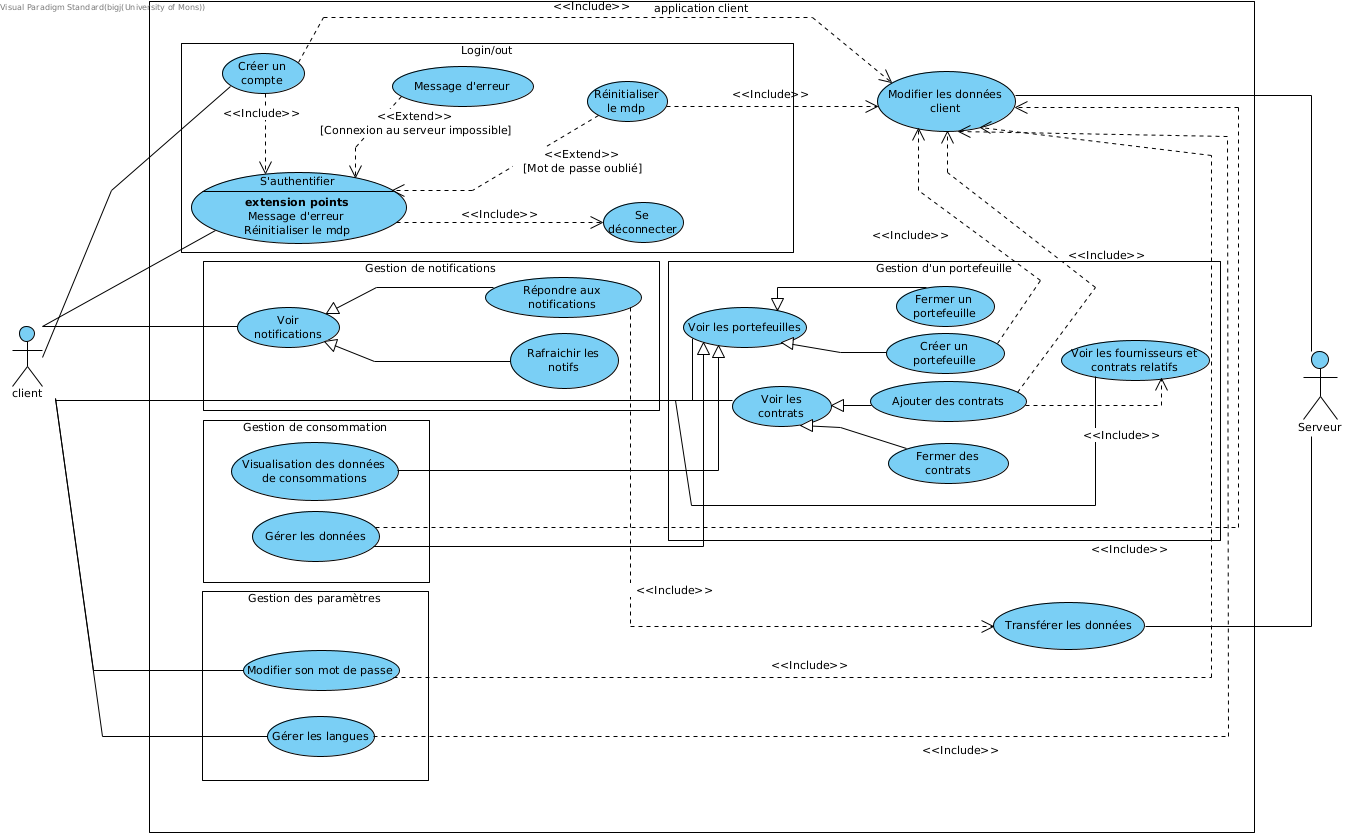
\includegraphics[width = 1\textwidth]{Base/use_case/img/client.png}
\end{figure}

\newpage

\subsection{Fournisseur}

\begin{flushleft}
Pour le fournisseur, les principales différences résident dans le fait qu’il n’y aura plus les sections « Voir les portefeuilles » et « Voir les contrats » mais « Voir ses clients » et « Voir les contrats clients ».
\end{flushleft}

\begin{flushleft}
Dans la même optique que pour la gestion d’un portefeuille chez le client, le fournisseur une fois sur la section « Voir ses clients » sera apte à ajouter ou supprimer un client, voir les données de ses clients ainsi que les gérer.
\end{flushleft}

\begin{flushleft}
Ce dernier aura, de plus, la possibilité d’ajouter ou fermer des contrats et changer les paramètres des contrats/propositions sur « Voir les contrats clients ».
\end{flushleft}

\begin{figure}[h]
\centering
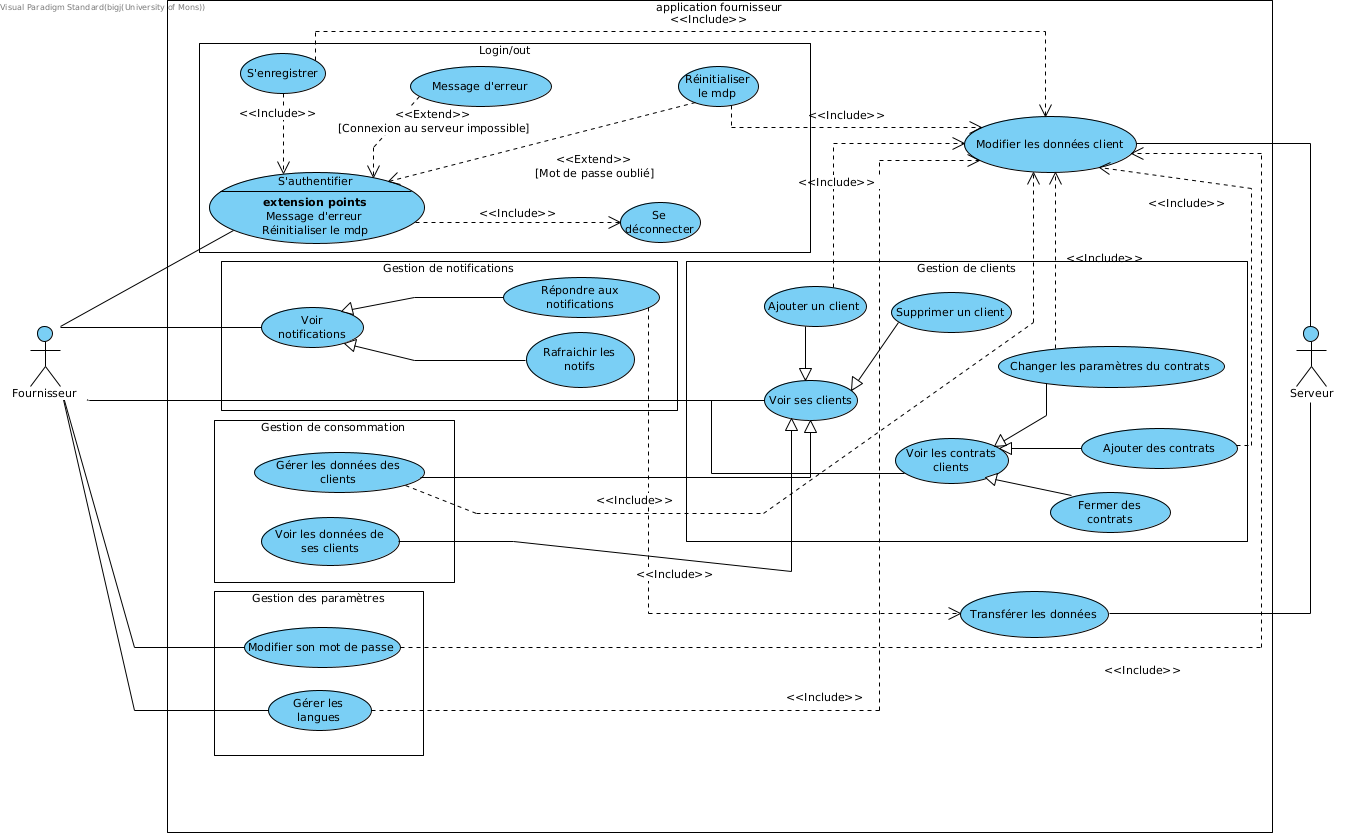
\includegraphics[width = 1\textwidth]{Base/use_case/img/fournisseur.png}
\end{figure}

\section{Interaction overview diagrams}

\subsection{Introduction}

\begin{flushleft}
Nous avons réalisé nos interaction overview diagrams sur base de nos use cases diagrams. 
Ce qui nous a permis de détailler la structure de ces diagrammes intuitivement.
\end{flushleft}

\begin{flushleft}
Ces derniers permettront d’obtenir une idée globale du parcours des utilisateurs sur l’application ainsi que les fonctionnalités leur étant disponibles.
\end{flushleft}

\begin{flushleft}
Nous décrirons donc deux applications, l’application « client » et l’application « fournisseur » et de nouveau, nous verrons apparaître des points communs entre ces dernières.
\end{flushleft}

\newpage
\subsection{Points communs}

\begin{enumerate}[1.]
\item  \textbf{Système de logs}:\newline 

Une fois que l’utilisateur arrivera sur l’application, plusieurs choix s’offriront à lui. Soit ce dernier est nouveau et il peut donc s’enregistrer en respectant les conditions qui lui sont imposées telles qu’une adresse mail valide, vérifiée par une demande de confirmation, et inexistante sur l’application, la mention de son rôle sur l’application (client ou fournisseur), un mot de passe ayant un niveau de sécurité convenable et le choix de sa langue, soit, il possède déjà un compte et se connecte. \newline

Cependant, celui-ci pourra réinitialiser son mot de passe à l’aide d’un mail de confirmation ou réessayer de se connecter si lors de la vérification des données, les identifiants sont invalides.\newline

De plus, lorsque l’utilisateur sera connecté sur l’application, il aura la possibilité de se déconnecter s’il le souhaite.

\item \textbf{Menu représenté par un « grand » fork :}\newline

Une fois connecté, l’utilisateur aura accès à un menu reprenant la déconnexion, l’accès aux paramètres, les notifications et les éléments lui étant propres en fonction qu’il soit fournisseur ou client. \newline
Cette façon de penser nous semblait suffisamment intuitive pour que l’utilisateur puisse naviguer sur l’application facilement. 
Nous avons également choisi de permettre un « retour » à ce menu lorsque nous sommes dans les sections le composant.

\item \textbf{Accès aux paramètres :}\newline

Une fois sur l’onglet des paramètres, plusieurs choix s’offrent à lui : 

\begin{enumerate}[a)]

\item Gérer les langues : plus précisément, il pourra en ajouter, en choisir une qui sera sa langue favorite et de changer la langue actuelle de l'application comme expliqué précédemment dans les Use cases diagrams.

\item Modifier son mot de passe : pour ce faire, l’utilisateur recevra un mail de confirmation permettant de le changer en toute sécurité.
\end{enumerate}

\item \textbf{Les notifications :}\newline
Une fois sur cette section, l’utilisateur pourra répondre à ses notifications, c’est-à-dire, marquer comme lues les contrats, les accepter, les refuser ou encore de voir leurs détails à savoir les données relatives à ces derniers. \newline

De surcroît, s’il le désire, ce dernier aura le droit de rafraichir ses notifications par lui-même sans attendre que cela se réalise automatiquement.

\end{enumerate}

\newpage
\subsection{Accès à l'application pour les clients}

Lorsque d’un client voudra \textbf{voir ses portefeuilles}, \newline il retrouvera plusieurs fonctionnalités :

\begin{enumerate}[1.]
\item Créer un portefeuille
\item Fermer un portefeuille
\item Visualisation des données de consommation
\item Gérer les données
\end{enumerate}

\begin{enumerate}[-]
\item \textbf{Créer un portefeuille : }\newline

Cette première option permettra au client comme son nom l’indique de créer un portefeuille. \newline
Dans cette optique, il devra rentrer le nom et l’adresse du portefeuille, le code EAN et ajouter les contrats liés.

\item \textbf{Fermer un portefeuille :}\newline

Cela donnera la possibilité au client de clôturer un portefeuille, une fois qu’il n’en aura plus d’utilité.

\item \textbf{Visualisation des données de consommation :}\newline

Le client pourra observer les valeurs associées à sa consommation, ainsi que les contrats étant liés à ces dernières.

\item \textbf{Gérer les données :} \newline
Il sera également apte à les modifier, c’est-à-dire, renouveler ses données de consommation et ajouter, modifier ou supprimer les contrats étant associés à un portefeuille.\newline
Grâce à cette option, ce dernier aura pleinement la main sur ses portefeuilles et aura la faculté de les reformer à sa guise.
\end{enumerate}

\newpage

\begin{flushleft}
Le menu offre en outre la possibilité de \textbf{voir les contrats} ou plus précisément de voir ses contrats, l’utilisateur sera donc en mesure de, d’ :
\end{flushleft}
\begin{enumerate}[1.]
\item Ajouter des contrats
\item Fermer des contrats
\end{enumerate}

\begin{enumerate}[-]
\item \textbf{Ajouter des contrats :}\newline

Le client se retrouvera alors sur la page des \textbf{fournisseurs et contrats relatifs} répertoriant tous les contrats qu’il ne possède pas encore et les verra en plus amples détails avant de les ajouter s’il le désire.

\item \textbf{Fermer des contrats :}\newline

Cela lui donnera la possibilité de clôturer un contrat s’il trouve cela plus judicieux.\newline

L’ajout et la fermeture de contrats impliquera une \textbf{notification} sur l’application du fournisseur en question.\newline

Nous avons décidé de laisser la possibilité au client de voir les fournisseurs et contrats relatifs sans forcément passer par la liste de ses contrats afin de lui permettre un accès plus rapide.
\end{enumerate}

\newpage

\begin{figure}[h]
\centering
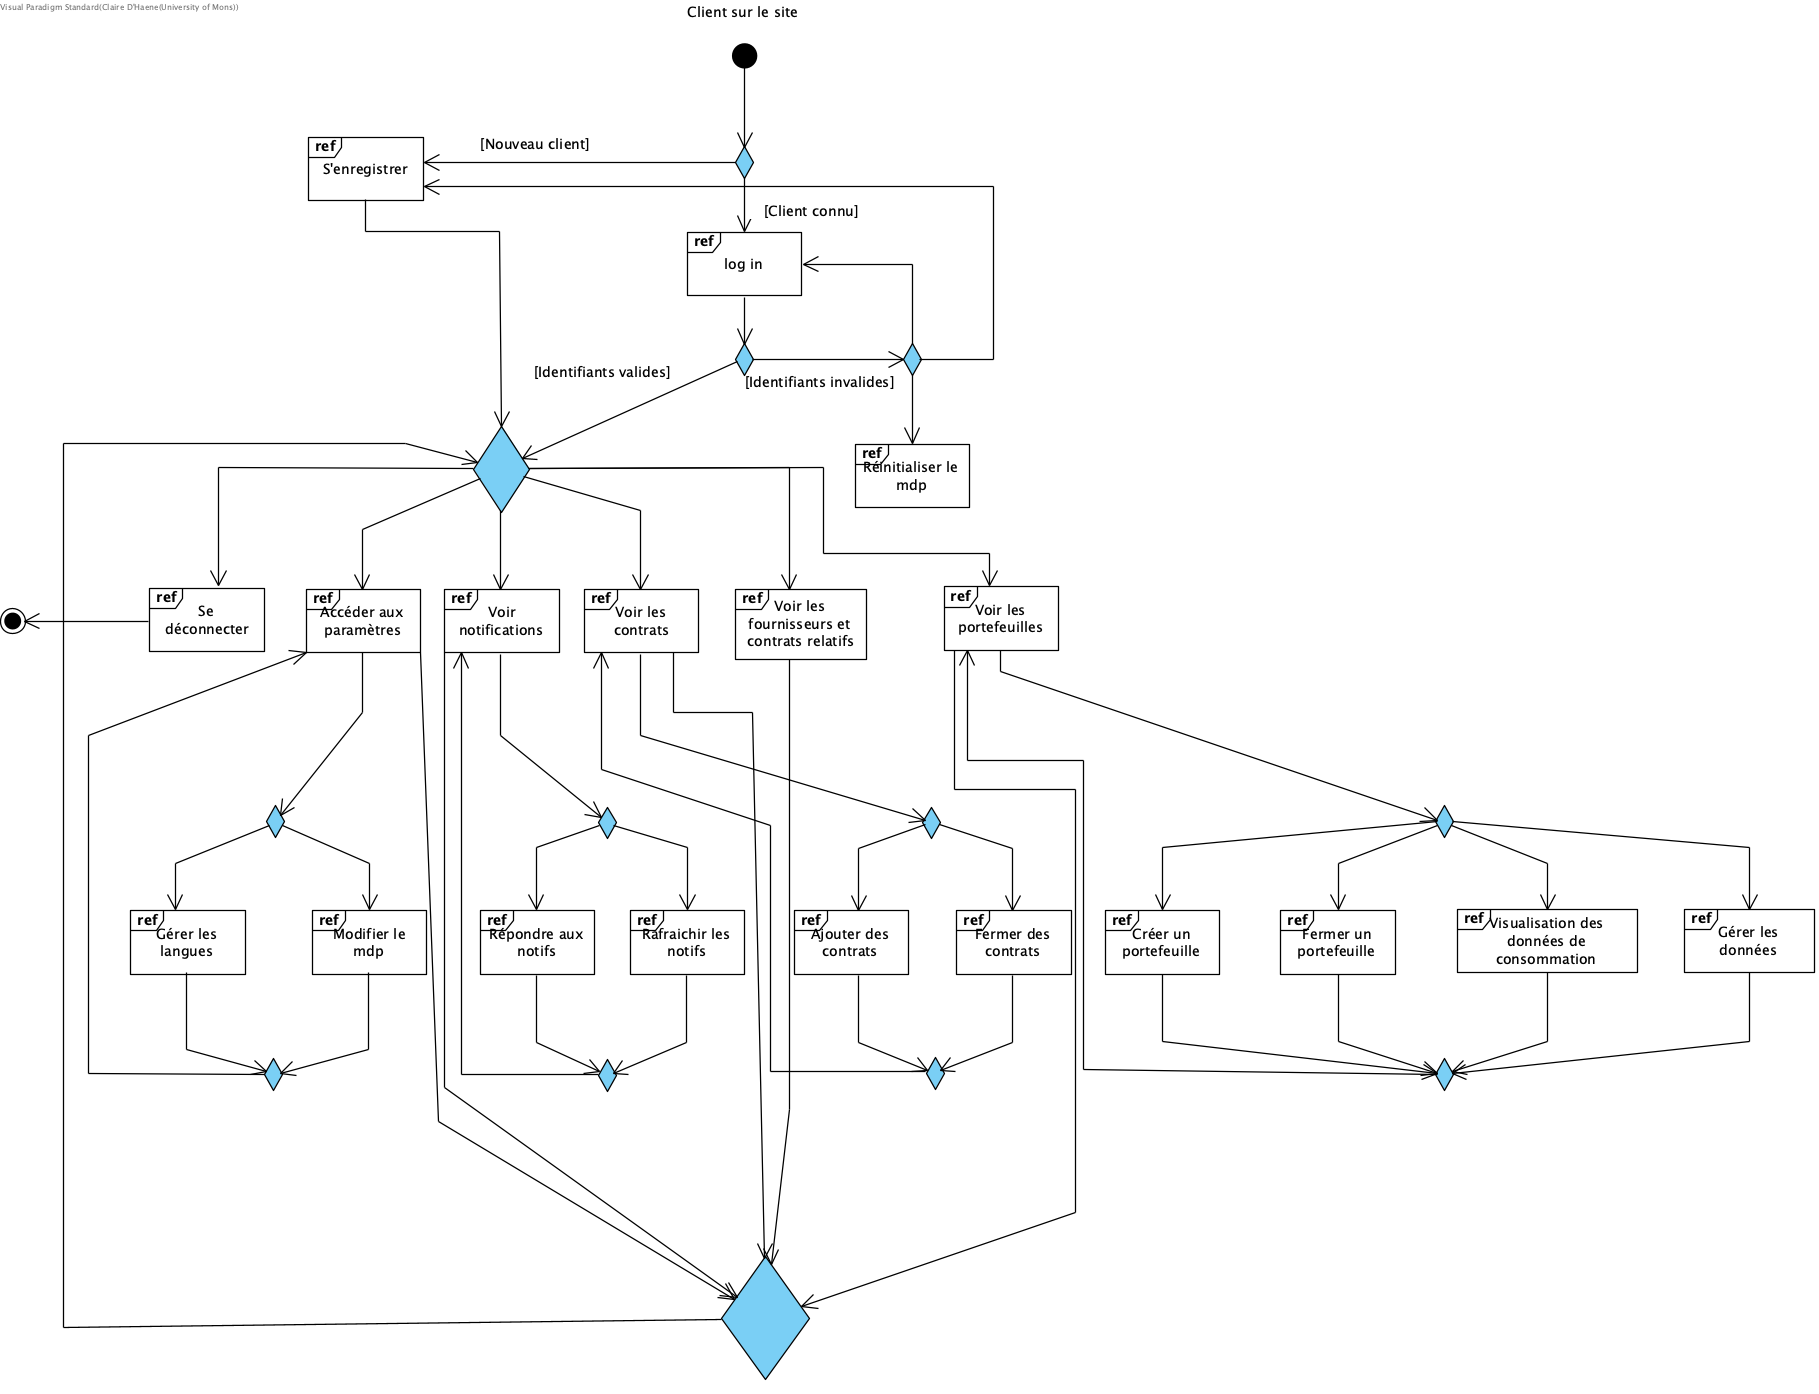
\includegraphics[width = 1\textwidth]{Base/overview/img/overview-client.png}
\end{figure}

\newpage

\subsection{Accès à l'application pour les fournisseurs}

Au moment où le fournisseur accèdera à l’onglet \newline « \textbf{Voir les contrats clients} », plusieurs choix s’offriront à lui :
\begin{enumerate}[1.]
\item Ajouter des contrats
\item Fermer des contrats
\item Changer les paramètres des contrats
\end{enumerate}

\begin{enumerate}[-]
\item \textbf{Ajouter des contrats :} \newline

Cette option permettra au fournisseur d’ajouter de nouveaux contrats qu’il aura créés aux contrats déjà existants en spécifiant les valeurs leur relatives (prix, type de fourniture et compteurs).


\item \textbf{Fermer des contrats : }\newline

Cela lui donnera la possibilité de clôturer un contrat, une fois qu’il n’en aura plus d’utilité.

\item \textbf{Changer des contrats : }\newline

Le fournisseur sera apte à changer les termes du contrat s’il trouve cela approprié.\newline
Évidemment comme pour la fermeture de contrats, le changement sera notifié au client.
\end{enumerate}

\newpage
\begin{flushleft}
De plus, le fournisseur sera à même de « \textbf{Voir ses clients} » de manière distincte, plus précisément, ce dernier retrouvera une liste de ses clients avec les contrats leur étant associés :
\end{flushleft}
\begin{enumerate}[1.]
\item Ajouter un client
\item Supprimer un client
\item Voir les données de ses clients
\item Gérer les données de ses clients
\end{enumerate}

\begin{enumerate}[-]

\item \textbf{Ajouter un client : }\newline

Ce dernier aura la capacité d’ajouter un client en l’associant à un de ses contrats en particulier.

\item \textbf{Supprimer un client :}\newline

Cela donnera la possibilité au fournisseur de clôturer tous les contrats actifs avec un client, s’il est d’avis que cela est nécessaire.

\item \textbf{Visualisation des données de ses clients :}\newline

Celui-ci pourra observer les valeurs associées aux contrats de ses clients, ainsi que leur consommation.

\item \textbf{Gérer les données de ses clients : }\newline

Le fournisseur aura également la capacité de les modifier, c’est-à-dire, modifier, ajouter ou supprimer les contrats étant associés à un client.\newline

Grâce à cette option, ce dernier aura pleinement la main sur ses clients et aura la faculté de les gérer à sa guise.\newline

L’ajout, la modification et la fermeture de contrats impliquera une notification sur l’application du client en question.

\end{enumerate}

\newpage

\begin{figure}[h]
\centering
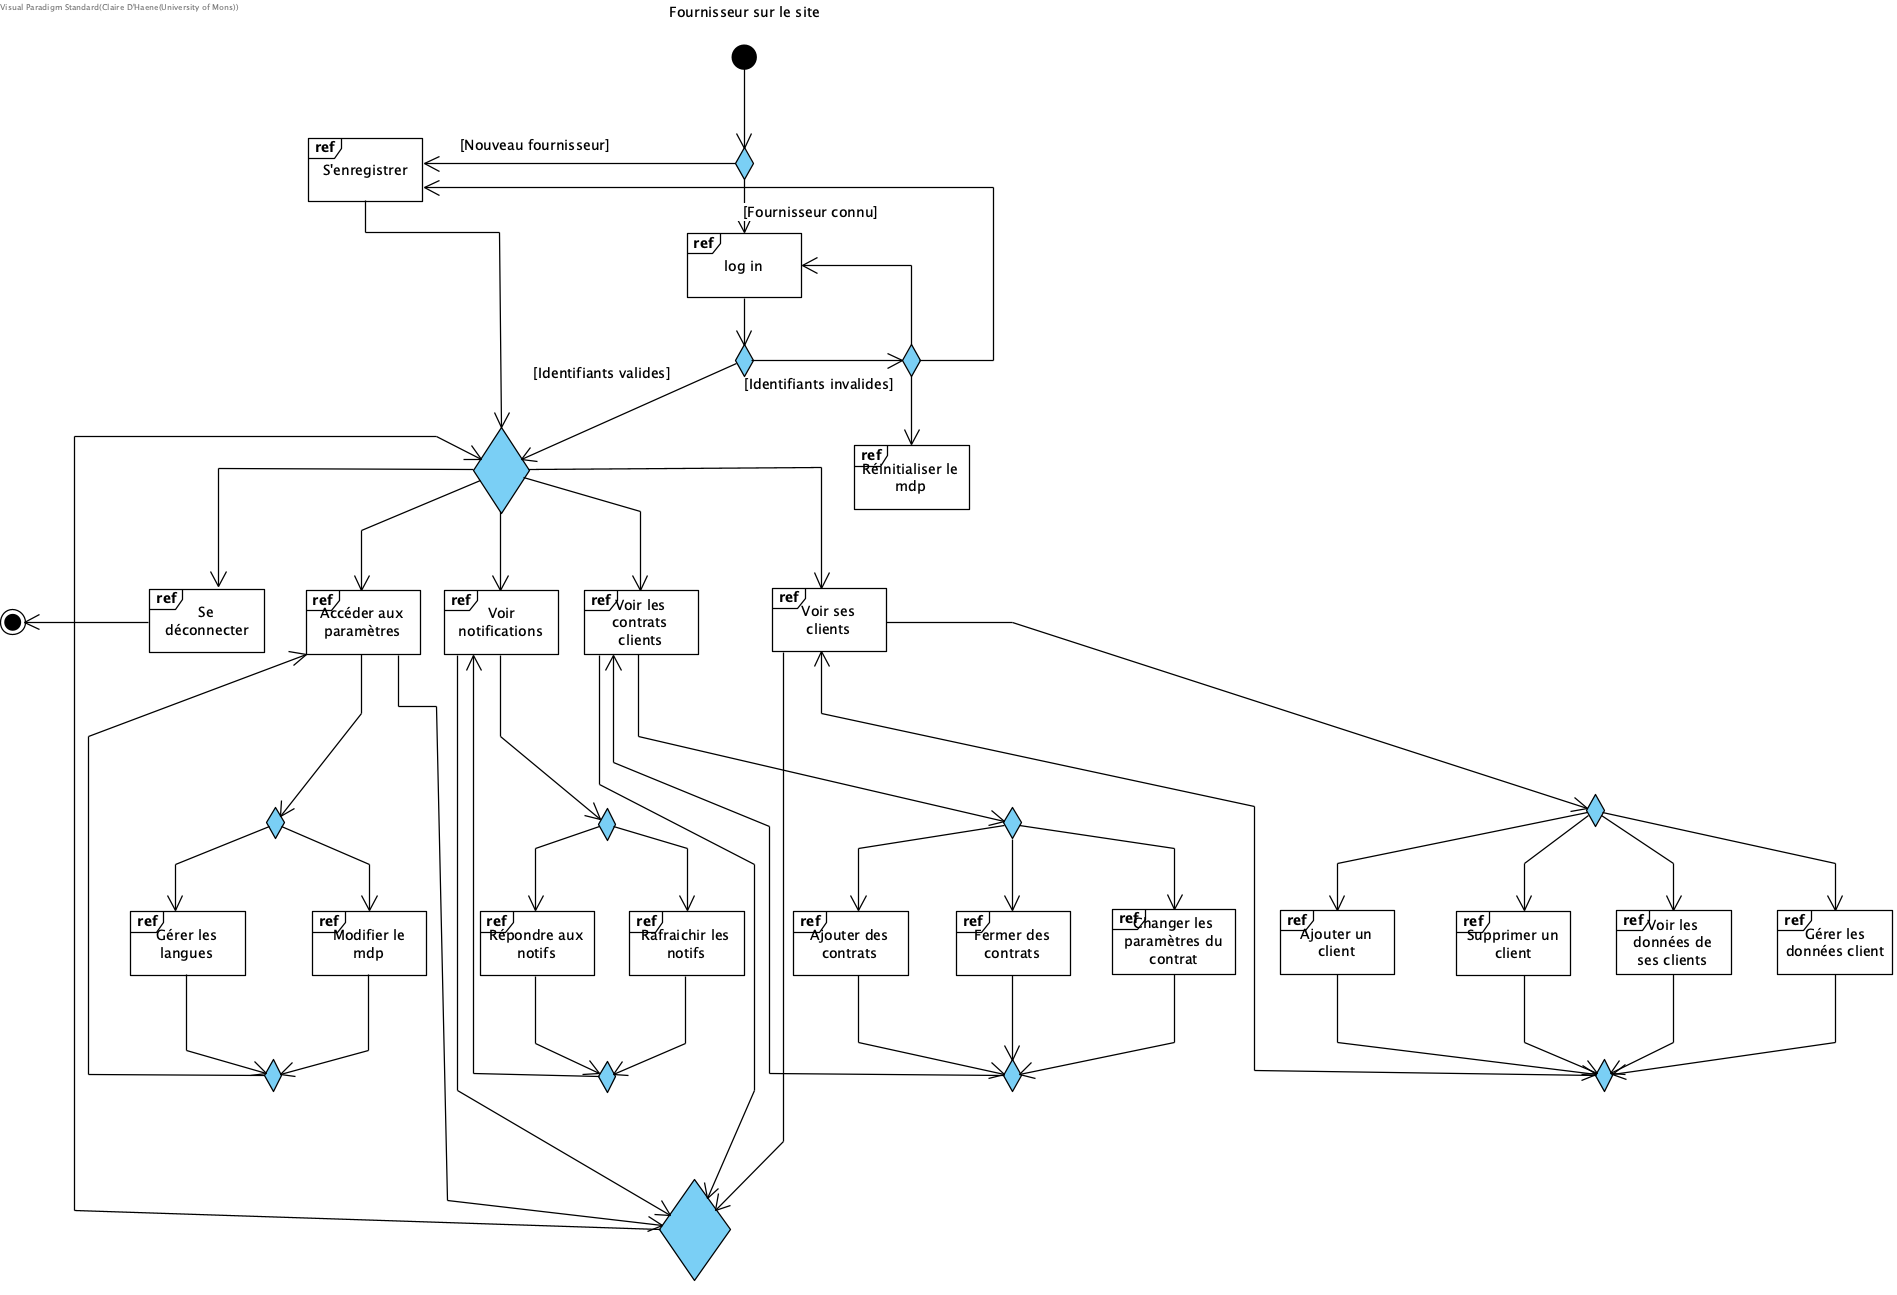
\includegraphics[width = 1\textwidth]{Base/overview/img/overview-fournisseur.png}
\end{figure}
\section{Entity relationship diagram}
\subsection{préambule}
\begin{flushleft}
Dans cette partie, nous allons parler de la modélisation de la base de donnée. Chaque sous-section parlera d'une relation. Dans ces sous-sections, nous parlerons du fonctionnement de certains attributs et nous définirons nos clés primaires et étrangères.
\end{flushleft}

\begin{flushleft}
De manière générale, nous avons fait en sorte d'obtenir le moins de redondance possible entre les différentes relations pour convenir au mieux à la 3NF\footnote{ \url{https://en.wikipedia.org/wiki/Third\_normal\_form}}.
\end{flushleft}
\subsection{utilisateur}
\begin{flushleft}
Nous partons du principe qu'un fournisseur et un client sont avant tout des utilisateurs de l'application. De ce fait, les deux personnes auront un identifiant "id"("u" + 9 digits). Cet identifiant représente la quantième personne qui a été inscrite. Par exemple, si je suis le premier utilisateur alors j'aurai l'identifiant : u000000000.
\end{flushleft}

\begin{flushleft}
A noter que le mot de passe sera stocké dans la base de données après avoir été "hashé" par l'algorithme bcrypt\footnote{\url{https://fr.wikipedia.org/wiki/Bcrypt}} pour éviter toute fuite dans le cas où la base de donnée serait compromise.
\end{flushleft}

\begin{flushleft}
PK(utilisateur) = \texttt{id}
\end{flushleft}

\begin{flushleft}
FK(utilisateur) REFS fournisseur = \texttt{id}

FK(utilisateur) REFS client = \texttt{id}
\end{flushleft}
\newpage
\subsection{langue}
\begin{flushleft}
Dans cette relation, nous posons que l'utilisateur peut avoir plusieurs langues. De ce fait, nous avons une clé primaire composée. 
\end{flushleft}

\begin{flushleft}
De plus, la langue enregistrée peut être une langue préférée (1 si c'est le cas, 0 sinon). 
\end{flushleft}

\begin{flushleft}
Ensuite, un attribut binaire \texttt{langue\_actuelle} est stocké. Cet attribut nous permet de savoir quelle langue l'utilisateur est en train d'utiliser ou a utilisé pendant sa dernière session (1 si c'est le cas, 0 sinon). 
\end{flushleft}

\begin{flushleft}
PK(langue) = \texttt{id} et \texttt{langue\_enregistrée}
\end{flushleft}

\begin{flushleft}
FK(langue) REFS utilisateur = \texttt{id}
\end{flushleft}
\subsection{client}
\begin{flushleft}
Du coté de la relation "client", nous y trouvons un seul attribut. Cela nous permet d'avoir un utilisateur ayant aucun portefeuille.
\end{flushleft}

\begin{flushleft}
PK(client) = \texttt{id\_client}
\end{flushleft}
\subsection{portefeuille}
\begin{flushleft}
L'adresse sera définie comme : nomdeville-nomderue-numérodemaison. 
\end{flushleft}

\begin{flushleft}
PK(portefeuille) = \texttt{adresse}
\end{flushleft}

\begin{flushleft}
FK(portefeuille) REFS client = \texttt{id\_client}
\end{flushleft}
\subsection{contrat du portefeuille}
\begin{flushleft}
 Dans "contrat du portefeuille" et pour toute autre relation, \texttt{id\_contrat} sera défini comme ceci : "c" + quantième contrat créé.
\end{flushleft}

\begin{flushleft}
PK(contrat du portefeuille) = \texttt{adresse} et \texttt{id\_contrat}
\end{flushleft}

\begin{flushleft}
FK(contrat du portefeuille) REFS portefeuille = \texttt{adresse}
\end{flushleft}
\subsection{fournisseur}
\begin{flushleft}
Un fournisseur sera perçu avec son identifiant. De même que le client, un fournisseur aura la possibilité de n'avoir aucun contrat ce qui justifie le fait qu'il n'y ait qu'un seul attribut dans la relation.
\end{flushleft}

\begin{flushleft}
PK(fournisseur) = \texttt{id\_fournisseur}
\end{flushleft}
\subsection{proposition}
\begin{flushleft}
Cette section correspondra aux offres du fournisseur avec tous les paramètres qui seront associés. Nous posons qu'un nom d'offre ne peut être unique par rapport à plusieurs fournisseurs. De ce fait, nous avons une clé primaire composée. L'attribut \texttt{nom\_proposition} sera du type : "p" + nom que le fournisseur aura donné.
\end{flushleft}

\begin{flushleft}
A noter que la localisation sera définie par un binaire de taille 3: le premier bit sera la région Wallonne, le second sera la région flamande et le troisième la région Bruxelles-Capitales. Comme exemple, 101 dira que le contrat sera disponible dans la région Wallonne et Bruxelles-Capitales .Du coté des autres types binaires, 1 sera vrai et 0 faux. 
\end{flushleft}

\begin{flushleft}
De plus, certains paramètres seront dépendants d'autres paramètres. Comme exemple, nous pouvons dire qu'il ne sera pas possible d'avoir  un prix différent entre les heures pleines et les heures creuses si le type d'énergie est l'eau ou qu'on a un compteur mono-horaire.
\end{flushleft}

\begin{flushleft}
Enfin, si nous avons que le prix est le même pendant les heures creuses et les heures pleines. Il sera donc inutile de conserver une heure bien précise (\texttt{début\_heures\_creuses} et \texttt{début\_heures\_pleines}\footnote{format: entier tel que les deux premiers digits seront l'heure et les minutes pour les derniers} pourront être nuls).
\end{flushleft}

\begin{flushleft}
PK(proposition) = \texttt{nom\_proposition} et \texttt{id\_fournisseur}
\end{flushleft}

\begin{flushleft}
FK(proposition) REFS fournisseur = \texttt{id\_fournisseur}
\end{flushleft}
\subsection{contrat du fournisseur}
\begin{flushleft}
PK(contrat du fournisseur) = \texttt{id\_contrat} et \texttt{id\_fournisseur}
\end{flushleft}

\begin{flushleft}
FK(contrat du fournisseur) REFS fournisseur = \texttt{id\_fournisseur}
\end{flushleft}
\subsection{contrat}
\begin{flushleft}
La table contrat contiendra tous les éléments typiques d'un contrat tels que le fournisseur, le client, la proposition,ect,...
\end{flushleft}

\begin{flushleft}
A noter que la date de fermeture peut être nulle. Cela conviendra à un contrat à durée indéterminée.
\end{flushleft}

\begin{flushleft}
PK(contrat) = \texttt{id\_contrat}
\end{flushleft}

\begin{flushleft}
FK(contrat) REFS contrat du fournisseur = \texttt{id\_fournisseur} et \texttt{id\_contrat}

FK(contrat) REFS proposition = \texttt{nom\_proposition}

FK(contrat) REFS contrat du portefeuille = \texttt{adresse} et \texttt{id\_contrat}

FK(contrat) REFS compteur = \texttt{ean}
\end{flushleft}
\newpage
\subsection{compteur}
\begin{flushleft}
Dans cette section, nous représentons le compteur associé à un contrat. Le compteur sera identifié par le code EAN. 
\end{flushleft}

\begin{flushleft}
PK(compteur) = \texttt{ean}
\end{flushleft}
\subsection{consommation}
\begin{flushleft}
Dans la consommation, nous pouvons noter qu'il est possible qu'un client n'ai rien consommé durant la journée. De ce fait, \texttt{consommation\_journalière} peut être mis à 0. On a aussi posé qu'un
client ne pouvait consommer plus de 30 kw/heure par jour\footnote{source : \url{https://shrinkthatfootprint.com/average-household-electricity-consumption/}} ce qui nous permet de restreindre la taille de \texttt{consommation\_journalière} à 3 digits.
\end{flushleft}

\begin{flushleft}
PK(consommation) = \texttt{ean} et \texttt{date}
\end{flushleft}

\begin{flushleft}
FK(consommation) REFS compteur = \texttt{ean}
\end{flushleft}

\subsection{notification}
\begin{flushleft}
Les notifications seront représentées par un identifiant("n" + quantième notification créée).
\end{flushleft}

\begin{flushleft}
En plus de ça, un contexte relativement court sera posé jusqu'à plus ample information.
\end{flushleft}

\begin{flushleft}
Enfin, un binaire permettra de savoir de qui vient la notification. 1 si c'est le fournisseur, client sinon.
\end{flushleft}

\begin{flushleft}
PK(notification) = \texttt{id\_notification}
\end{flushleft}

\begin{flushleft}
FK(notification) REFS fournisseur = \texttt{id\_fournisseur}

FK(notification) REFS client = \texttt{id\_client}
\newpage

\end{flushleft}
\subsection{schéma}
\begin{figure}[h]
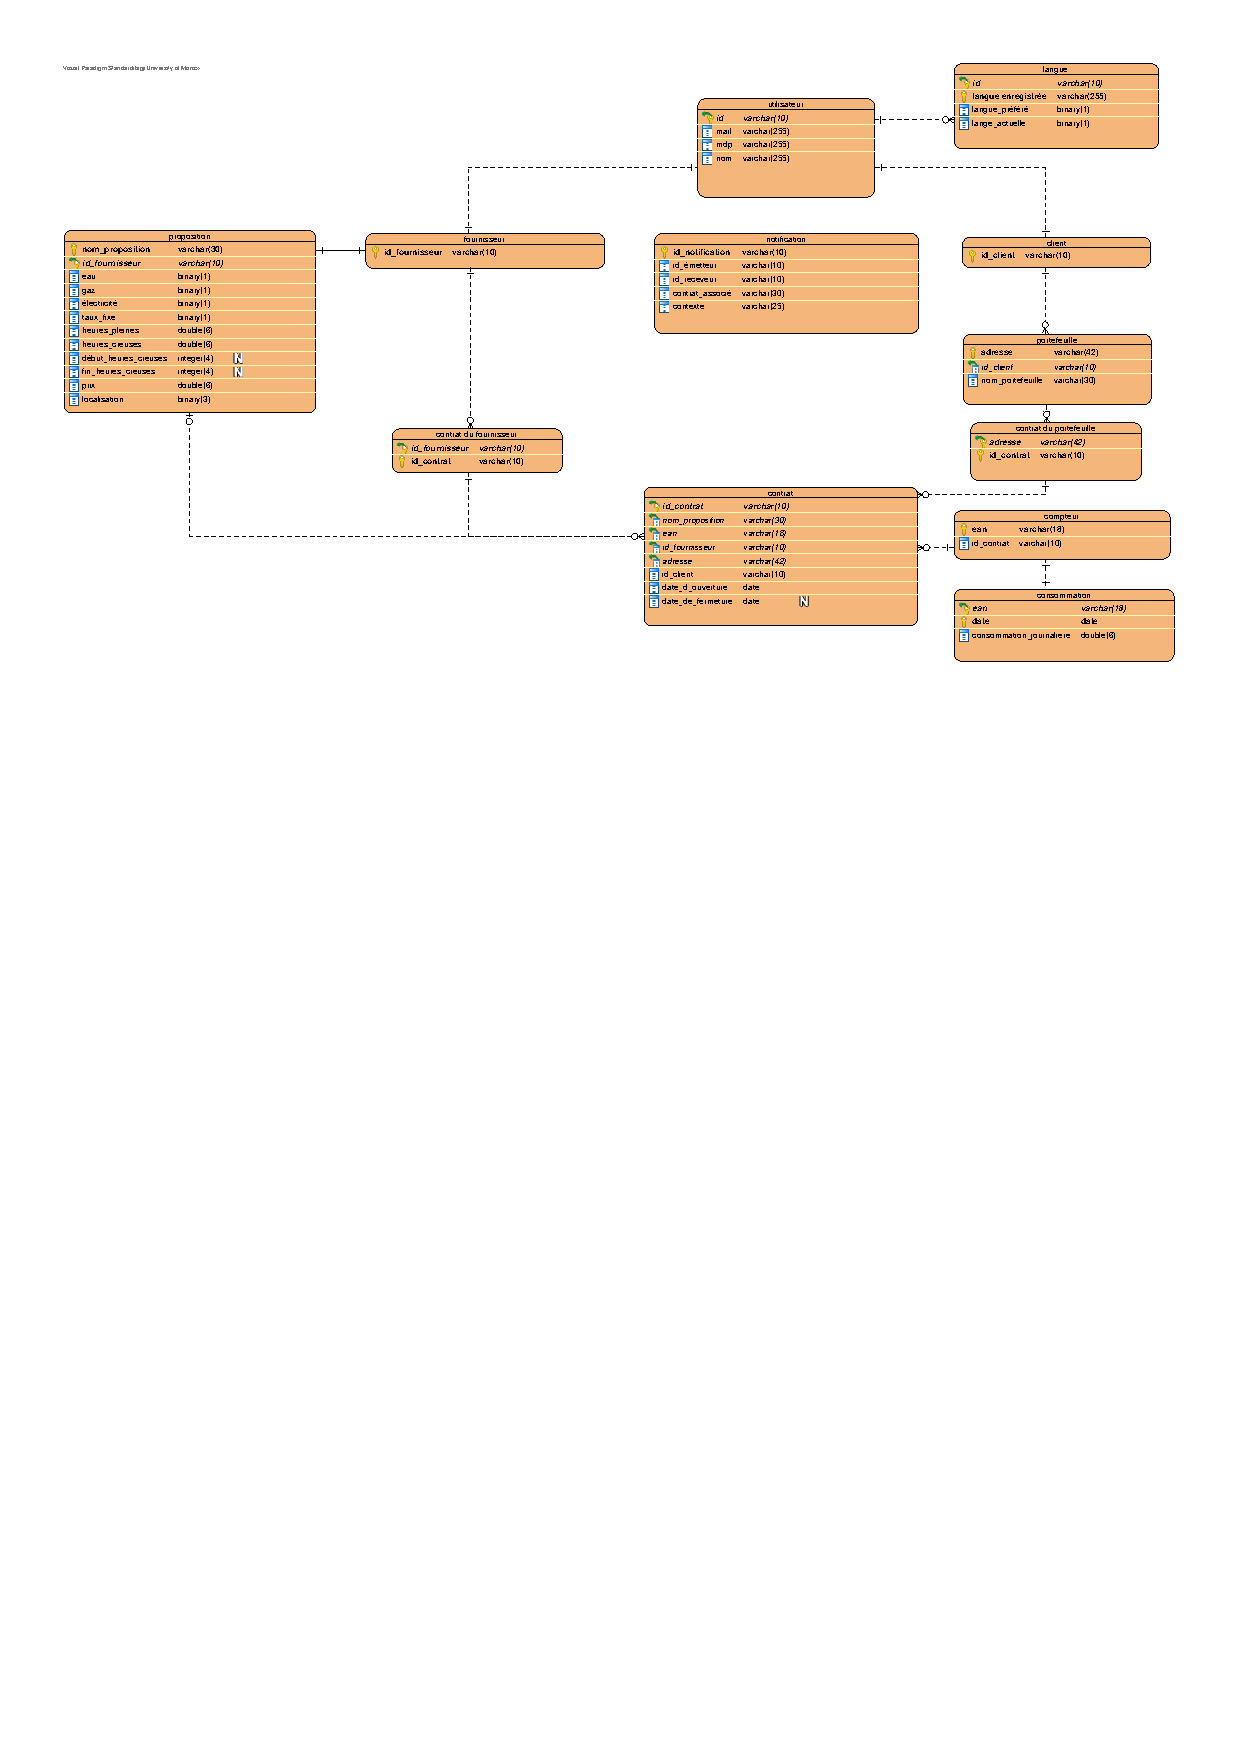
\includegraphics[scale=0.5]{Base/bdd/img/bdd.pdf}
\end{figure}

\section{Class diagram}

\subsection{Introduction}
\begin{flushleft}
Étant donné la taille du projet, nous avons évidemment décidé de séparer le projet en plusieurs parties. Au niveau du serveur, nous pouvons compter 3 grandes parties.
\end{flushleft}

\begin{enumerate}[-]
\item Le package API
\item Le package database
\item Le package dataObject
\end{enumerate}

\begin{flushleft}
En outre, il y a également la classe de base nommé App. Nous en reparlerons par après.
\end{flushleft}
\newpage
\subsection{Le package API}

\begin{flushleft}
Ce package contient toute la partie logique de l'ApiRest. Pour créer le serveur API nous avons décidé d'utiliser le framework Vertx\footnote{\url{https://thierry-leriche-dessirier.developpez.com/tutoriels/java/creer-API-rest-vertx-5-minutes/}}, nous expliquerons notre choix dans le rapport sur l'implementation. Pour créer une ApiRest, nous avons d'abord besoin d'une classe (MyApi) qui hérite de AbstractVerticle (une classe abstraite venant du package vertx). MyApi permet de lancer le serveur à l'aide de la méthode start.
\end{flushleft}

\begin{flushleft}
Avant de la lancer, il faut d'abord configurer les routes de notre API. Notre API étant conséquente, nous avons décidé de la séparer en 4 sous-routes (parties distinctes).
\end{flushleft}

\begin{enumerate}[a)]
\item \textbf{LogApi:}\newline
Celle-ci va être utilisée pour toutes les opérations liées au login. Autrement dit, pouvoir se connecter ou se déconnecter, créer un compte et réinitialiser son mot de passe en cas d'oubli. Nous avons aussi rajouté une méthode getCode pour envoyer un code de vérification par mail lorsque l'utilisateur veut créer un compte ou pour réinitialiser son mot de passe.
\item \textbf{ClientApi:}\newline
Celle-ci va être utilisée pour toutes les requêtes liées aux clients lorsqu'ils seront connectés. Ils pourront effectuer toutes les opérations qu'ils souhaitent au niveau du portefeuille ainsi que voir tous leurs contrats et pour finir voir toutes les propositions des fournisseurs ou une en particulier. Le client pourra évidemment proposer de conclure un contrat en fonction des propositions précédemment vues.
\item \textbf{ProviderApi:}\newline
Celle-ci va être utilisée pour toutes les requêtes liées aux fournisseurs lorsqu'ils seront connectés. Ils pourront effectuer toutes les opérations qu'ils souhaitent au niveau de leurs propositions mais également voir tous les clients de l'application, tous leurs clients ou un client en particulier. Contrairement au client, il a la possibilité de supprimer une ou toutes les données de consommations liées à un contrat. De plus, tout comme le client, il pourra proposer de conclure un contrat à n'importe quelle client à partir de l'une de ces propositions.
\item \textbf{CommonApi:}\newline
Celle-ci va être utilisée pour toutes les requêtes qui sont communes aux clients et aux fournisseurs lorsqu'ils seront connectés. On y trouve les méthodes pour les langues, pour les notifications et pour les données de consommations. Il y a également une méthode pour voir un contrat en particulier et une qui permet de changer de mot de passe.
\end{enumerate}
\newpage
\begin{flushleft}
Chacune de ces parties vont donc créer une sous-route grâce à la méthode getSubRouter car elles implémentent toutes l'interface Router. Et c'est donc dans la méthode start de MyApi que toutes ces sous-routes vont être rassemblées pour finalement lancer le serveur API.
\end{flushleft}

\begin{flushleft}
Notez que toutes les méthodes qui vont être appelées par l'API sont en privé car seul le serveur API peut les appeler et elles ont  le même argument (routingContext) car c'est cette variable qui contient la requête de l'utilisateur ainsi que le corps de la requête. Et c'est également par cette variable que nous pourrons répondre à l'utilisateur.
\end{flushleft}

\begin{flushleft}
Constatez également que ces quatre parties héritent d'une classe abstraite nommée AbstractToken. Comme son nom l'indique, elle va gérer les tokens. Autrement dit, lorsqu'un utilisateur se connecte, on va créer un token et c'est grâce à ce token qu'il pourra envoyer des requêtes aux classes clientApi, ProviderApi et CommonApi. Le token se supprimera automatiquement après un certain délai (15 minutes) ou lorsque quand l'utilisateur se déconnectera.
\newline
Notez que si le token est expiré, l'utilisateur devra se reconnecter.
\end{flushleft}

\subsection{Le package database}

\begin{flushleft}
Le package database contient toutes les méthodes qui vont communiquer avec la base de données. Une grande partie de celles-ci ont exactement le même nom que dans le package API puisqu’elles sont contenues dans la suite du programme. L'utilisateur envoie une requête à l'API, en fonction de la requête, la bonne méthode est appelée et appellera la méthode de database portant le même nom pour accéder aux données. Pour séparer le programme, nous avons divisé  cette partie en trois. Nous retrouvons donc une classe mère et deux classes filles.
\end{flushleft}

\begin{flushleft}
CommonDB est la classe mère de ce package, elle reprend toutes les méthodes communes aux clients et aux fournisseurs comme son nom l'indique. Outre les méthodes de l'API, nous retrouvons également les méthodes createNotification, deleteNotification et createContract car elles devront être appelées à la suite d'une requête et non directement. Nous avons aussi décidé d'ajouter les méthodes createId, getDataOfTable et deleteDataOfTable car ce sont des actions qui seront souvent utilisées et que nous pouvons donc généraliser.
\end{flushleft}

\begin{flushleft}
ClientDB et ProviderDB sont les deux classes enfants, elles s'occupent respectivement du côté client et du côté fournisseur comme leurs noms l'indiquent. Elles héritent de la classe CommonDB pour avoir accès à certaines méthodes comme par exemple createId, getDataOfTable et deleteDataOfTable. Notez qu'au niveau du client nous avons rajouté une méthode walletIsEmpty qui permet de savoir si un portefeuille du client est vide.
\end{flushleft}

\subsection{Le package dataObject}

\begin{flushleft}
Le package dataObject contient toutes les classes représentant un objet, c'est-à-dire:
\end{flushleft}

\begin{enumerate}[-]
\item Les portefeuilles.
\item Les contrats.
\item Les clients (du point de vue des fournisseurs).
\item Les propositions (que les fournisseurs ont créées).
\item Les notifications.
\end{enumerate}

\begin{flushleft}
Remarquez également que nous avons rajouter une classe TypeEnergy pour énumerer tous les types d'énergies.
\end{flushleft}

\begin{flushleft}
Nous avons décidé de créer ces objets pour transférer facilement les données. En effet toutes les classes ne contiennent que des attributs avec des assesseurs à quelques exceptions près. Notez que nous aurions donc pu mettre les variables en final mais nous avons préféré laisser comme ça car dans le cas contraire, nous aurions eu des constructeurs vraiment longs. Ces classes seront donc instanciées lorsque nous recevrons un objet par l'API ou quand nous prendrons des données de la base de données pour facilement les envoyer à l'utilisateur en format json (io.vertx.core.json.Json).
\end{flushleft}

\begin{flushleft}
À l'exception de la classe notification, nous avons choisi de séparer chaque sorte d'objets en deux parties, une partie basique avec les informations primaires et une partie complète avec le reste des informations. Cela nous permet, lorsque l'utilisateur souhaite par exemple voir tous ces portefeuilles, d'envoyer seulement le nécessaire au lieu d'envoyer toutes les données en une fois. Ce n'est que lorsque l'utilisateur cliquera sur un portefeuille en particulier que nous enverrons toutes les données correspondant à celui-ci.
\end{flushleft}
\newpage
\subsection{La classe App}

\begin{flushleft}
La classe App est le début du programme. C'est elle qui est chargée de lancer le programme comme toutes applications java grâce à la méthode nommée "main". En effet, cette méthode va lancer l'API de la classe Myapi. Notez que nous n'avons pas directement lié ces deux classes entre elles car l'API se lance indirectement par le framework Vertx.
\end{flushleft}

\begin{flushleft}
La classe App contient également quelques méthodes statiques utilisées par les autres parties du projet. Ce sont ces méthodes qui s'occupent de la partie mail du projet, notamment "sendEmail" qui enverra un mail à un utilisateur qui souhaite créer un compte, réinitialiser son mot de passe ou bien le changer. Les autres méthodes s'occupent du "code". En effet, nous avons décidé que lorsqu'un utilisateur souhaite réaliser une des tâches précédentes, nous allons lui envoyer un code par mail avec quelques explications. Nous avons donc besoin d'une méthode pour générer le code aléatoirement, une pour vérifier que l'utilisateur a entré le bon code et pour finir une pour supprimer le code si l'utilisateur a mis trop de temps pour l'envoyer.
\end{flushleft}

\begin{flushleft}
En outre, pour envoyer un mail, nous utilisons l'API javaxmail.
\end{flushleft}

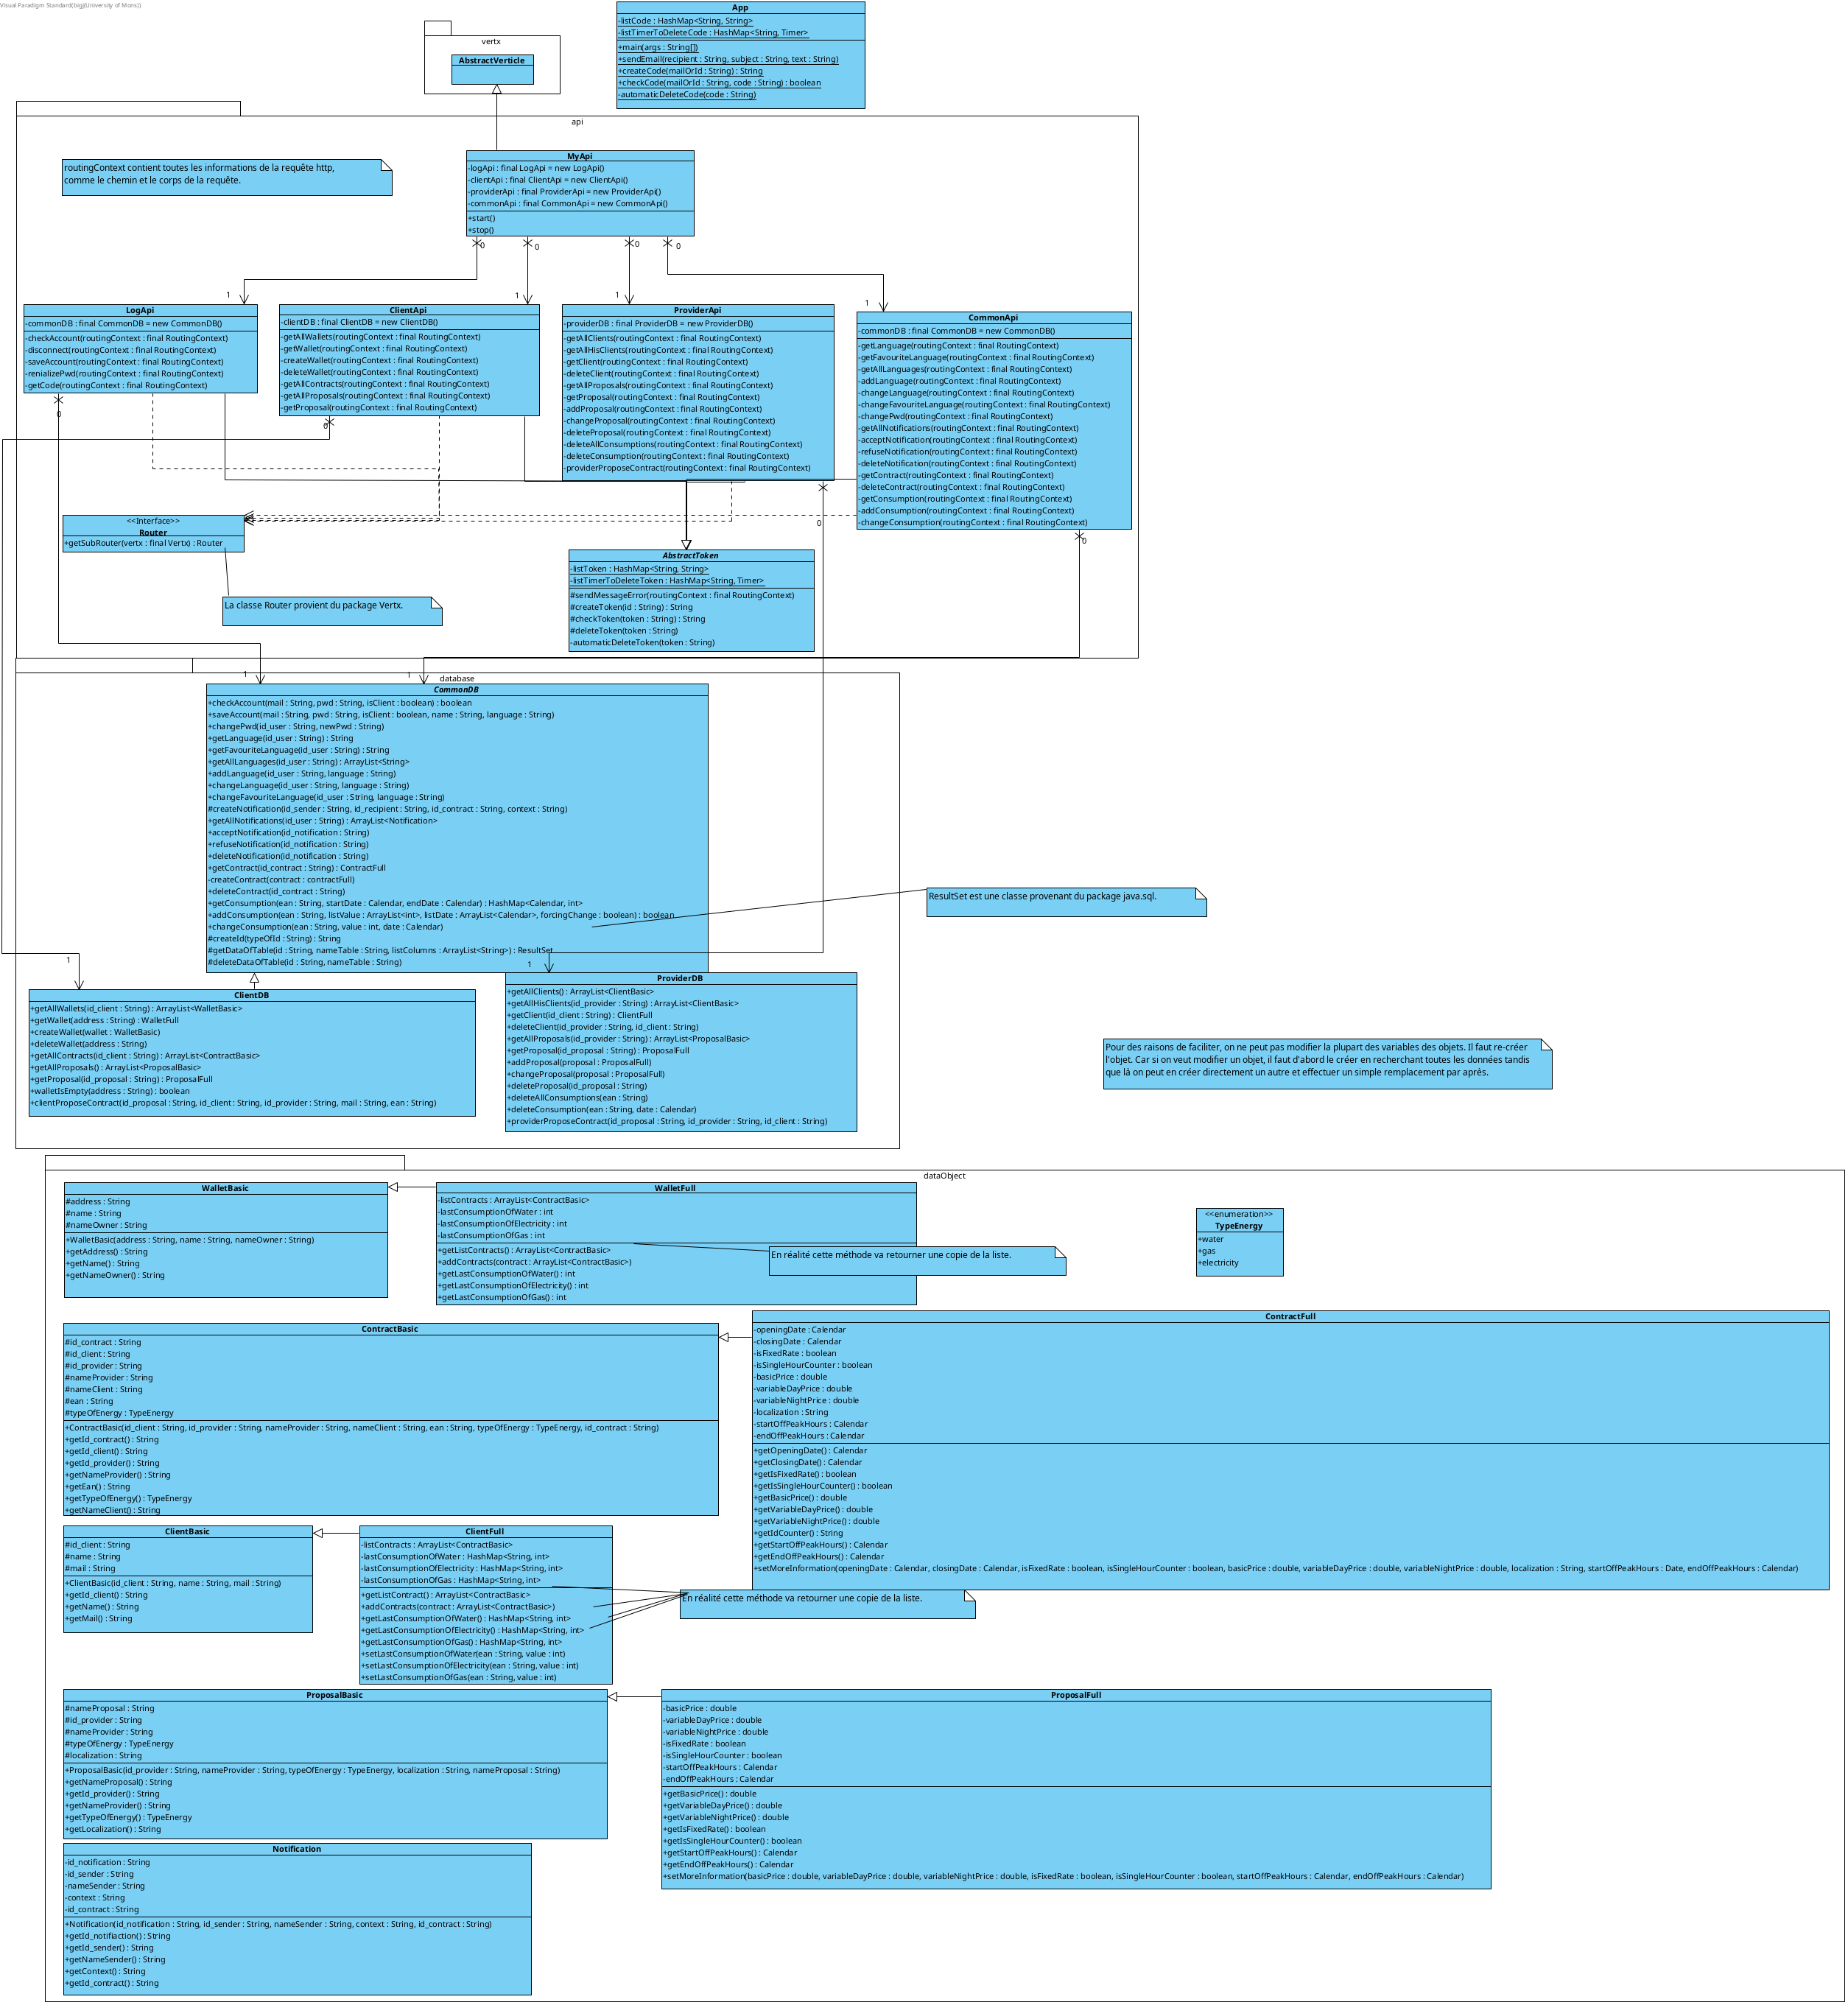
\includepdf[pages=-]{Base/classDiagram/img/classDiagram.png}

\section{Sequence diagrams}

\subsection{Introduction}

\begin{flushleft}
Les sequences diagrams nous permettent de détailler le chemin effectué lorsqu'un utilisateur souhaite intéragir avec l'application.
\end{flushleft}

\begin{flushleft}
Dans le but de permettre une meilleure compréhension de ces diagrammes, nous les avons séparés en trois parties.
\begin{enumerate}
\item Common
\item Client
\item Provider
\end{enumerate}
\end{flushleft}

\begin{flushleft}
Afin de les réaliser convenablement, nous sommes repartis de notre class diagram et nos Use cases diagrams et avons représenté l'interaction des méthodes avec l'API et la base de données.
\end{flushleft}

\begin{flushleft}
Avant de commencer, il est important de signaler dans le but d'éviter toute répétition, que la vérification du token s'effectuera pour chaque action lorsqu'un utilisateur est connecté.
\end{flushleft}

\begin{flushleft}
Si le token est bon, on continue le programme, sinon, on envoie un message d'erreur à l'aide de la méthode "sendMessageError".
\end{flushleft}

\begin{flushleft}
Pour rappel, l'utilisateur n'appelle pas directement les méthodes partant de sa lifeline mais utilise des requêtes de l'API. De plus, vous pouvez constater que dans le diagramme des classes, nous n'avons pas mis de type de retour aux méthodes de l'API. Cependant, dans les diagrammes de séquences, nous avons quand-même représenté une flèche de retour. Cela est dû au fait que pour retourner quelque chose à l'utilisateur, nous utilisons une méthode de la variable routingContext.
\end{flushleft}

\newpage
\subsection{Common}

\begin{flushleft}
Pour la partie commune aux clients et fournisseurs, nous retrouvons plusieurs Use Cases à décrire.
\end{flushleft}

\begin{enumerate}
\item Gérer les données
\item Gérer les langues
\item Modifier son mot de passe
\item Répondre aux notifications
\item S'authentifier
\item Visualisation des données de consommations
\item Voir les contrats
\item Voir notifications
\end{enumerate}

\newpage
\subsubsection{Gérer les données}

\begin{flushleft}
Nous pouvons gérer les données de deux manières. L'utilisateur peut ajouter une donnée de consommation ou en changer une.
\end{flushleft}

\begin{flushleft}
Pour ajouter une donnée, il suffit d'appeler la méthode addConsumption. Cette dernière peut écraser des données selon les paramètres utilisés. Lorsque des données sont écrasées, nous devons donc créer une notification pour prévenir l'autre utilisateur concerné par ce changement.
\end{flushleft}

\begin{flushleft}
Pour changer une donnée, il suffit d'appeler la méthode changeConsumption. Celle-ci change automatiquement une donnée, nous devons donc créer une notification pour prévenir l'autre utilisateur.
\end{flushleft}

\begin{figure}[h]
\centering
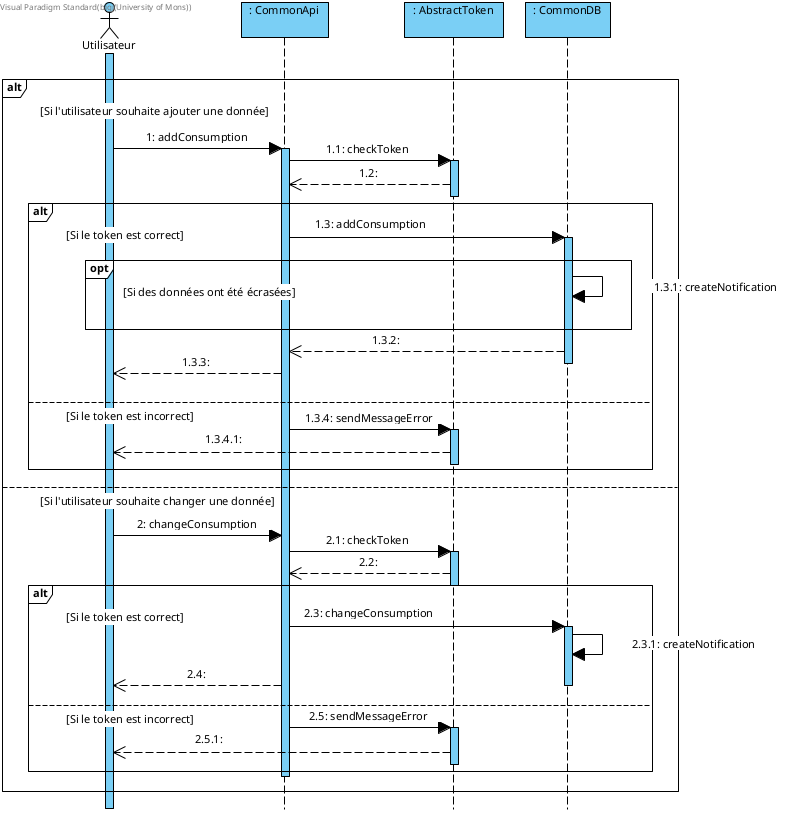
\includegraphics[width = 0.7\textwidth]{Base/sequence/img/common/Gérer les données.png}
\end{figure}

\newpage
\subsubsection{Gérer les langues}

\begin{flushleft}
Nous pouvons gérer les langues à plusieurs niveaux. L'utilisateur peut voir toutes ses langues, sa langue actuelle et sa langue préférée. En plus de cela, il peut ajouter une langue, changer sa langue actuelle ou encore changer sa langue favorite.
\end{flushleft}

\begin{flushleft}
Pour les trois premières fonctionnalités, le principe est le même. On appelle la méthode adéquate et celle-ci va t'être rappelée dans la partie base de donnée pour rechercher l'information désirée.
\end{flushleft}

\begin{flushleft}
Concernant les autres fonctionnalités, on appelle également la méthode du même nom dans la partie base de données. Remarquez que ces méthodes ne retournent rien.
\end{flushleft}

\begin{figure}[h]
\centering
\includegraphics[height = 1\textwidth]{Base/sequence/img/common/Gérer les langues.png}
\end{figure}

\newpage
\subsubsection{Modifier son mot de passe}

\begin{flushleft}
Pour modifier son mot de passe de manière sécurisée, nous passons par l'adresse mail de l'utilisateur pour être certains que ce soit bien celui-ci qui veuille changer le mot de passe. Pour se faire, il faut tout d'abord faire appel à la méthode getCode, cette dernière va appeler les méthodes createCode et sendEmail de la classe App.
\end{flushleft}

\begin{flushleft}
À noter que createCode va appeler automaticDeleteCode afin que le code se supprime automatiquement au bout d'un laps de temps au cas où l'utilisateur prendrait trop de temps ou n'utiliserait jamais ce code.
\end{flushleft}

\begin{flushleft}
L'utilisateur recevra donc par mail un code de vérification. Il pourra ensuite entrer le code et son nouveau mot de passe sur le site pour finalement appeler la méthode changePwd de l'API. Avant de le changer, nous utilisons la méthode checkCode d'App pour vérifier que le code est correct. Si c'est bien le cas, alors nous pouvons appeler changePwd de CommonDB pour changer le mot de passe. Dans le cas contraire, nous renvoyons évidemment un message d'erreur.
\end{flushleft}

\begin{figure}[h]
\centering
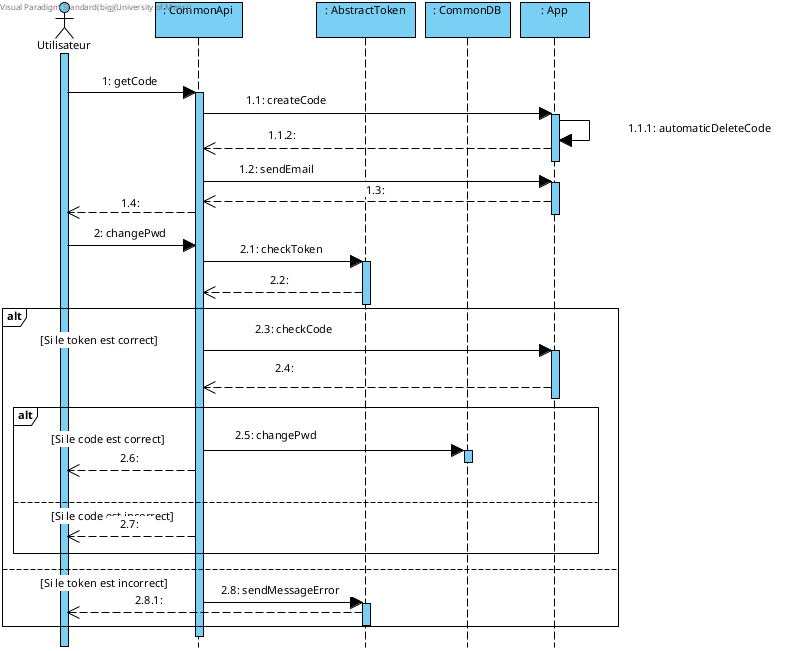
\includegraphics[height = 0.9\textwidth]{Base/sequence/img/common/Modifier son mot de passe.png}
\end{figure}

\newpage
\subsubsection{Répondre aux notifications}

\begin{flushleft}
Répondre aux notifications implique trois possibilités. L'utilisateur peut l'accepter ou la refuser dans le cas d'une demande de contrat ou bien dans les autres cas, noter la notification comme lue.
\end{flushleft}

\begin{flushleft}
Lorsqu'un utilisateur accepte une notification (une demande de contrat). Dans la partie base de données, nous commençons par créer un objet contractFull à partir de la proposition acceptée, ensuite nous faisons appel à la méthode createContract pour enregistrer le contrat. Nous pouvons donc supprimer la notification actuelle étant donné qu'elle vient d'être acceptée. Pour finir, nous créons une nouvelle notification pour informer à l'autre utilisateur que sa demande a été acceptée.
\end{flushleft}

\begin{flushleft}
Dans le cas d'une notification informative, l'utilisateur peut la marquer comme lue. Ce qui implique de la supprimer en appelant la méthode deleteNotification.
\end{flushleft}

\begin{figure}[h]
\centering
\includegraphics[height = 0.9\textwidth]{Base/sequence/img/common/répondre aux notifications.png}
\end{figure}

\newpage

\subsubsection{S'authentifier}

\begin{flushleft}
Lorsque l'utilisateur arrive sur la fenêtre de connexion. Deux cas de base sont possibles. Si l'utilisateur n'a pas de compte ou au contraire s'il en possède déjà un.
\end{flushleft}

\begin{flushleft}
Pour créer un compte, suivant le même principe que le changement de mot de passe. Un code va être crée et envoyé à l'adresse mail que l'utilisateur vient d'entrer grâce aux méthodes déjà expliquées ci-dessus. Quand l'utilisateur souhaite sauvegarder son compte, la méthode saveAcccount est invoquée. Après vérification du code, cette dernière est ré-appelée dans CommonDB pour sauvegarder le compte.
\newline
Suite à cela, Nous pouvons créer un token de connexion grâce à la méthode createToken de la classe abstraite AbstractToken et l'envoyer à l'utilisateur pour ses prochaines requêtes car en créant son compte, il s'est également connecté. Notez que lors de la création du token, nous appelons automaticDeleteToken pour limiter la durée de vie du token.
\end{flushleft}

\begin{flushleft}
Si l'utilisateur possède déjà un compte, nous vérifions les données de connexion grâce à checkAccount. Si les données sont correctes, nous pouvons créer un token et l'envoyer comme expliqué précédemment.
\end{flushleft}

\begin{flushleft}
Si l'utilisateur possède un compte mais ne parvient pas à se connecter. Il a la possibilité de réinitialiser son mot de passe. Le processus utilisé est le même que lors du changement de mot de passe expliqué précédemment.
\end{flushleft}

\begin{flushleft}
Une fois connecté, l'utilisateur peut de toute évidence se déconnecter en faisant appel à la méthode disconnect. Celle-ci servant juste à appeler deleteToken pour supprimer le token.
\end{flushleft}

\newpage
\begin{figure}[h]
\centering
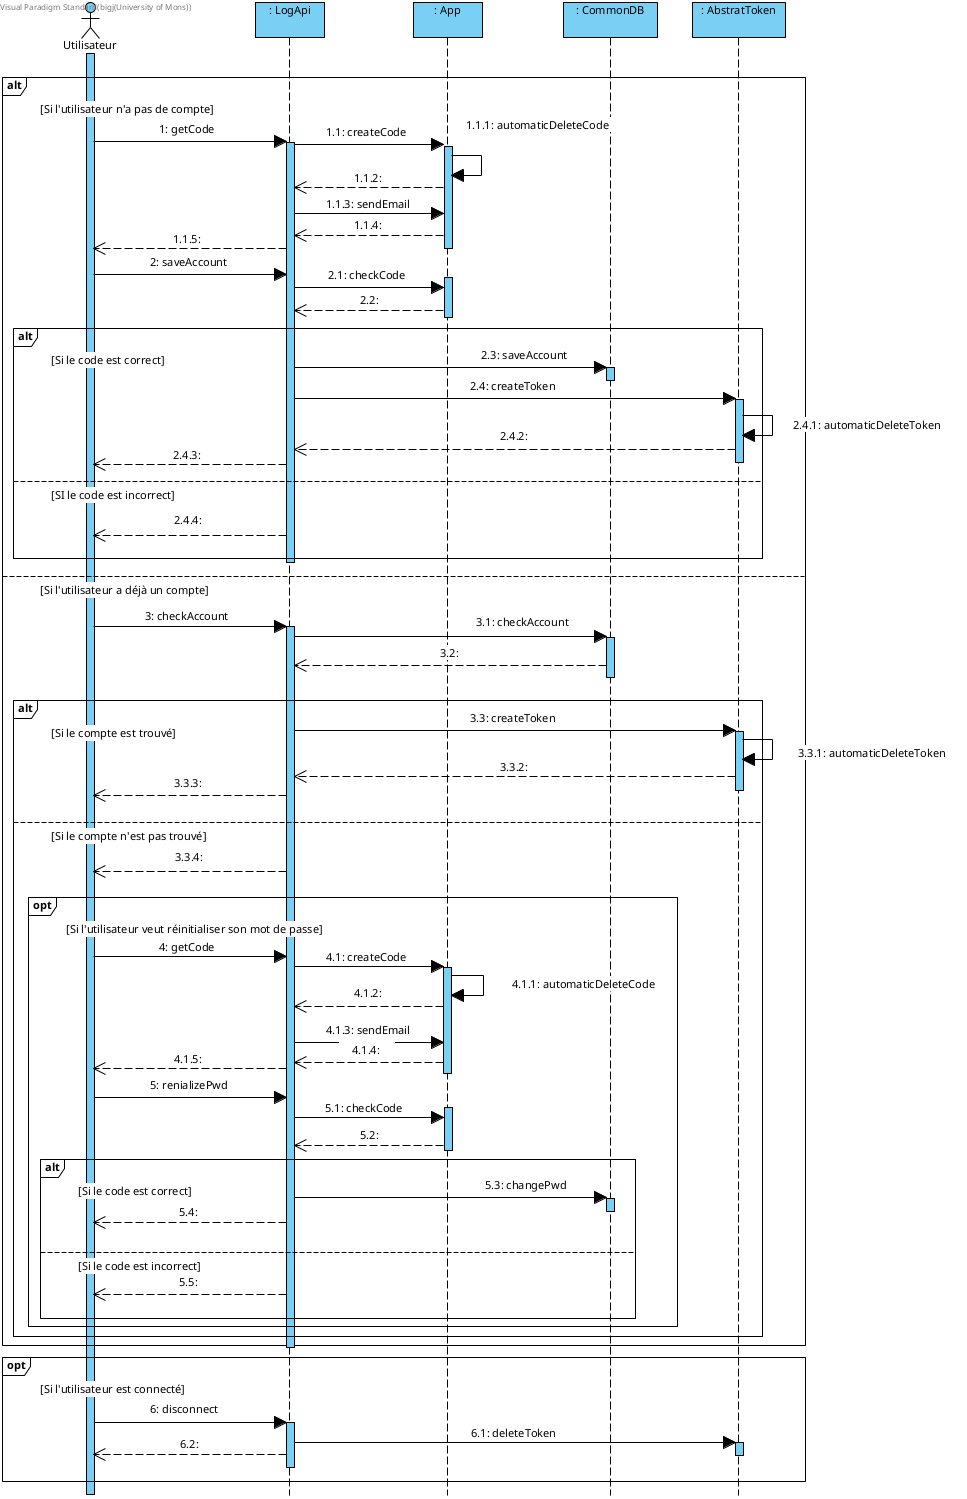
\includegraphics[height = 1\textwidth]{Base/sequence/img/common/S'authentifier.png}
\end{figure}

\newpage
\subsubsection{Visualisation des données de consommations}

\begin{flushleft}
Rien de plus simple. Nous invoquons la méthode getConsumption de l'API, ensuite elle est ré-appelée dans CommonDB pour récupérer les valeurs dans la base de données pour finalement les renvoyer.
\end{flushleft}

\begin{figure}[h]
\centering
\includegraphics[height = 1\textwidth]{Base/sequence/img/common/Visualisation des données de consommations.png}
\end{figure}

\newpage

\subsubsection{Voir les contrats}

\begin{flushleft}
Au niveau des contrats dans la partie commune, il est possible de voir un contrat en particulier ainsi que d'en supprimer un.
\end{flushleft}

\begin{flushleft}
Il suffit d'appeler la méthode getContract jusqu'à la base de données, nous pouvons ensuite créer un objet ContractFull pour facilement renvoyer les valeurs liées à cet objet. Notez qu'une fois envoyé, l'objet est détruit.
\end{flushleft}

\begin{flushleft}
Comme son nom l'indique, deleteContract permet de supprimer un contrat. Une fois son devoir accompli, cette méthode doit également créer une notification pour avertir l'autre utilisateur impliqué par cette suppression. Il n'est pas utile que cette méthode renvoie quelque chose.
\end{flushleft}

\begin{figure}[h]
\centering
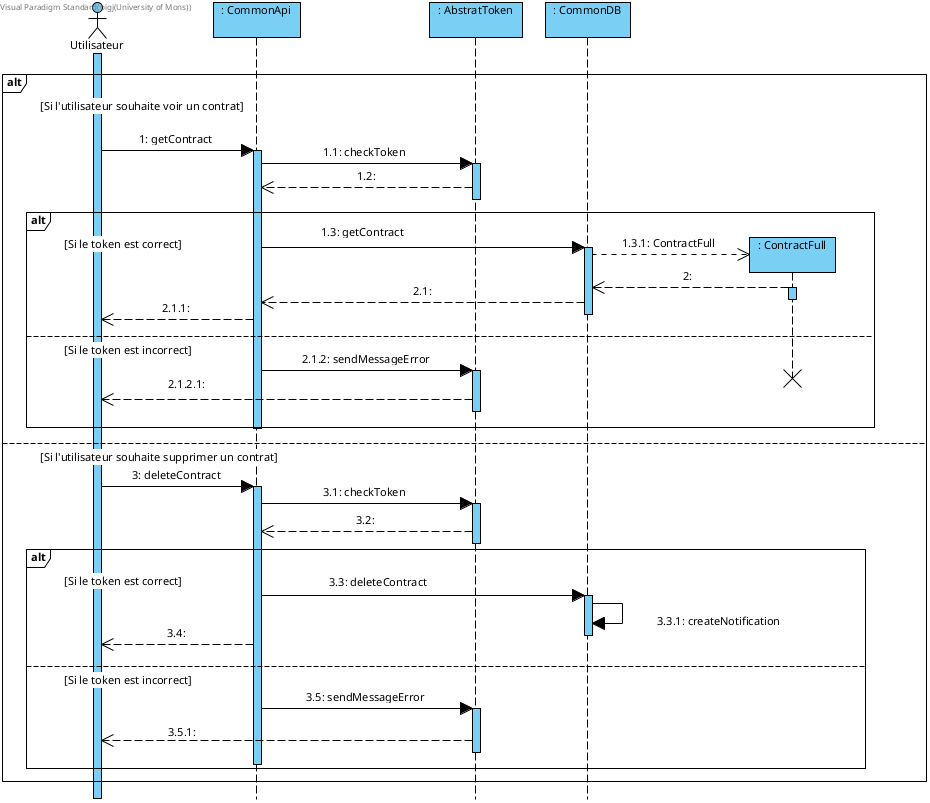
\includegraphics[height = 1\textwidth]{Base/sequence/img/common/Voir les contrats.png}
\end{figure}

\newpage

\subsubsection{Voir notifications}

\begin{flushleft}
Pour finir, l'utilisateur peut voir ses notifications. Pour cela, nous suivons toujours le même principe en appelant d'abord la méthode getAllNotifications au niveau de l'API et ensuite dans la partie base de données. Nous créons un objet Notification pour chaque notification stockée pour les envoyer dans une liste vers l'utilisateur. Tous les objets précédemment créés seront évidement supprimés à la suite de l'envoi de la liste.
\end{flushleft}

\begin{flushleft}
Notez que lorsque l'utilisateur rafraîchit les notifications, c'est cette même méthode qui est appelée.
\end{flushleft}

\begin{figure}[h]
\centering
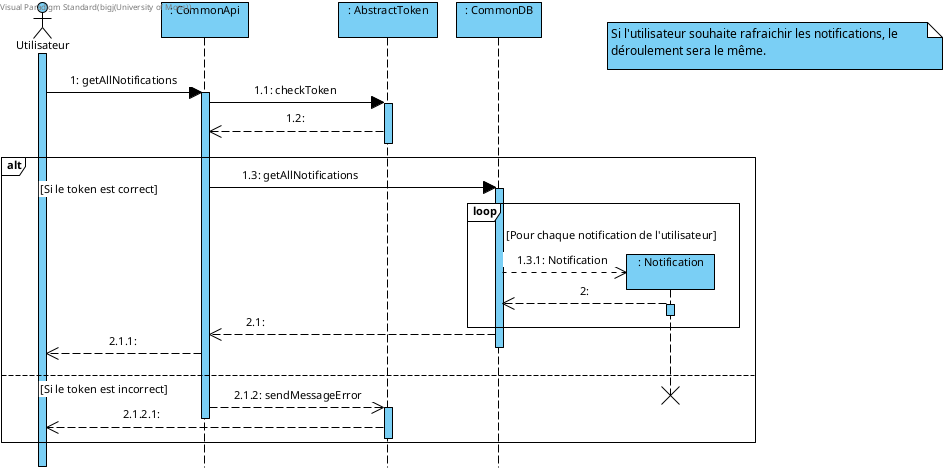
\includegraphics[height = 1\textwidth]{Base/sequence/img/common/Voir notifications.png}
\end{figure}

\newpage
\subsection{Client}

\subsubsection{Contrats}\label{CONTRATS}

\begin{flushleft}
Commençons par le Use Case \textbf{"Voir les contrats"}, nous appelons la méthode "getAllContract" de clientApi et ensuite, la méthode du même nom de ClientDB.
\end{flushleft}

\begin{flushleft}
Le but étant d'obtenir une ArrayList de "contractBasic", nous devons effecter une boucle afin de récupérer tous les "contractBasic".
\end{flushleft}

\begin{flushleft}
Une fois effectuée, nous renvoyons cette liste.
\end{flushleft}

\begin{figure}[h]
\centering
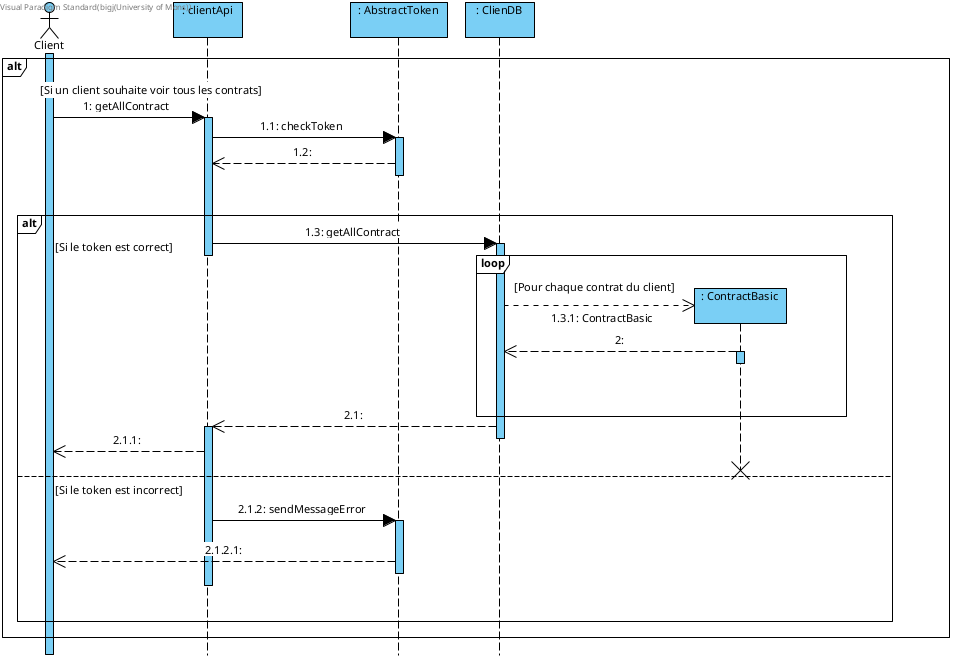
\includegraphics[height = 0.9\textwidth]{Base/sequence/img/client/Voir les contrats.png}
\end{figure}

\newpage

\subsubsection{Fournisseurs et
contrats relatifs}
\begin{flushleft}
Continuons avec l'Use Case \textbf{"Voir les fournisseurs et
contrats relatifs"}.
A cet effet, il y aura deux méthodes :
\end{flushleft}

\begin{enumerate}
\item getAllProposal si le client souhaite voir toutes les propositions.
\item getProposal si le client souhaite voir une proposition en particulier.
\end{enumerate}

\begin{flushleft}
Ces deux méthodes sont appelées une fois de clientApi et ensuite, une fois de ClientDB.
\end{flushleft}

\begin{flushleft}
Dans le cas de "getAllProposal", la valeur de retour est une ArrayList de "proposalBasic" donc nous utiliserons une boucle et dans le cas de "getProposal", nous devons simplement retourner une instance de "proposalFull".
\end{flushleft}

\begin{flushleft}
Concernant le Use Case \textbf{"Ajouter des contrats"}, nous appelons la méthode "clientProposeContract" de clientApi et ensuite, la méthode du même nom de ClientDB.
\end{flushleft}

\begin{flushleft}
Etant donné que cette dernière ne doit rien retourner, il n'y aura pas de valeur de retour.
\end{flushleft}

\newpage
\begin{figure}[h]
\centering
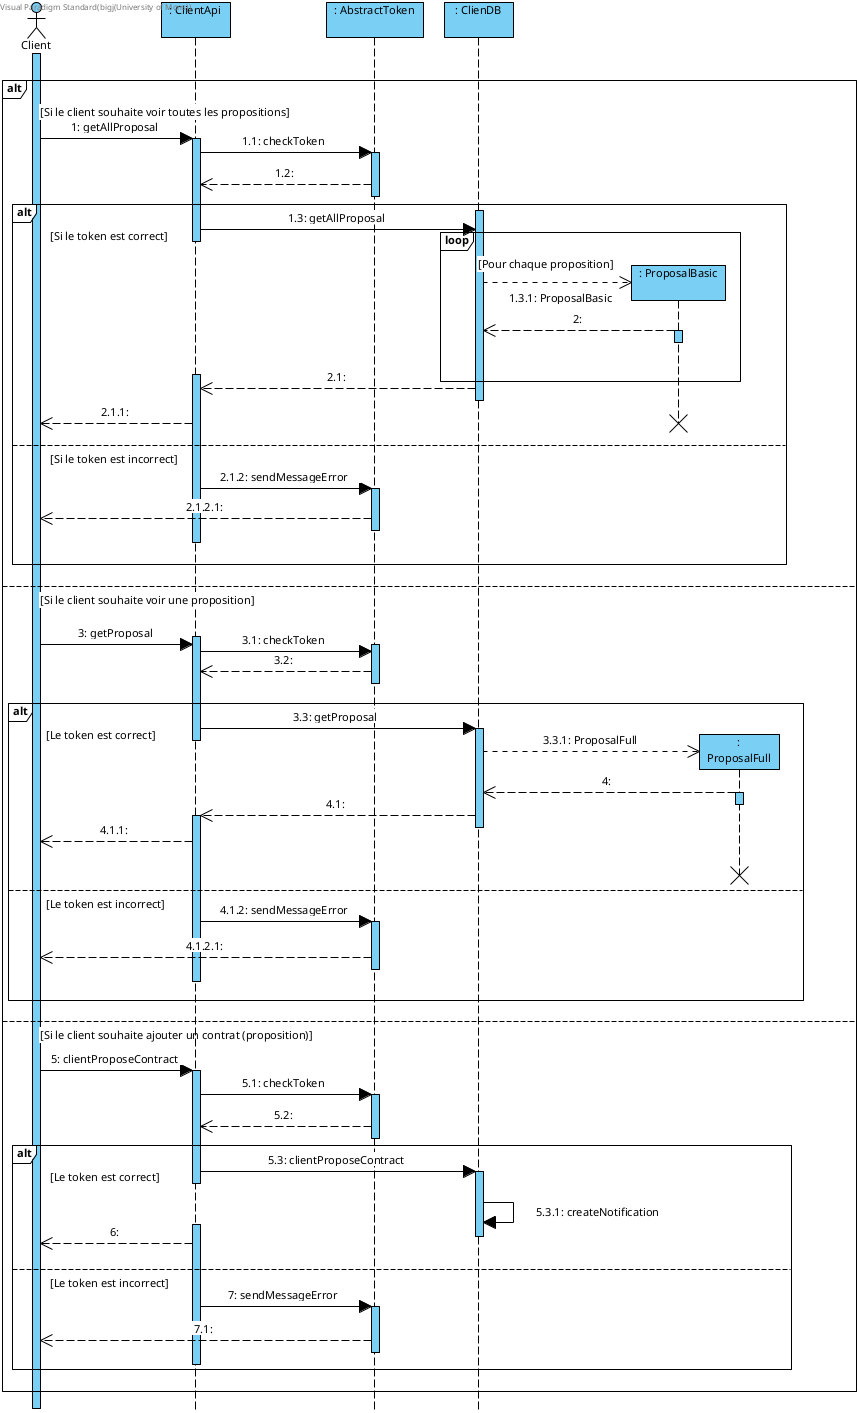
\includegraphics[height = 1.2\textwidth]{Base/sequence/img/client/Voir les fournisseurs et contrats relatifs.png}
\end{figure}

\newpage

\subsubsection{Portefeuilles}
\begin{flushleft}
L'Use case \textbf{"Voir les portefeuilles"} fonctionne de la même manière qu'expliqué précédemment pour "Voir les fournisseurs et contrats relatifs".
En effet, il y aura deux méthodes : 
\end{flushleft}
\begin{enumerate}
\item getAllWallet si le client souhaite voir tous les portefeuilles. On doit donc retourner une ArrayList de "walletBasic".
\item getWallet si le client souhaite voir un portefeuille en particulier. On doit donc retourner une instance de "walletFull".
\end{enumerate}

\begin{flushleft}
Passons maintenant aux Use Cases \textbf{"Créer un portefeuille"} et \textbf{"Fermer un portefeuille"}.
\end{flushleft}

\begin{flushleft}
Pour \textbf{créer un portefeuille}, nous appelons donc la méthode "createWallet" de clientApi et ensuite, la méthode du même nom de ClientDB.
\end{flushleft}

\begin{flushleft}
Nous créons une instance de "walletBasic", que nous devons enregistrer dans "ClientDB" avant de clôturer l'exécution de la méthode car il s'agit d'un nouveau portefeuille à stocker.
\end{flushleft}

\begin{flushleft}
Pour \textbf{supprimer un portefeuille}, nous appelons la méthode "deleteWallet" de clientApi.
\end{flushleft}
\begin{flushleft}
Cependant, avant d'appeler la méthode du même nom de ClientDB, nous devons vérifier que le portefeuille est vide.
\end{flushleft}
\begin{flushleft}
Si c'est le cas le portefeuille sera bien supprimé, sinon, on renverra une erreur.
\end{flushleft}

\newpage
\begin{figure}[h]
\centering
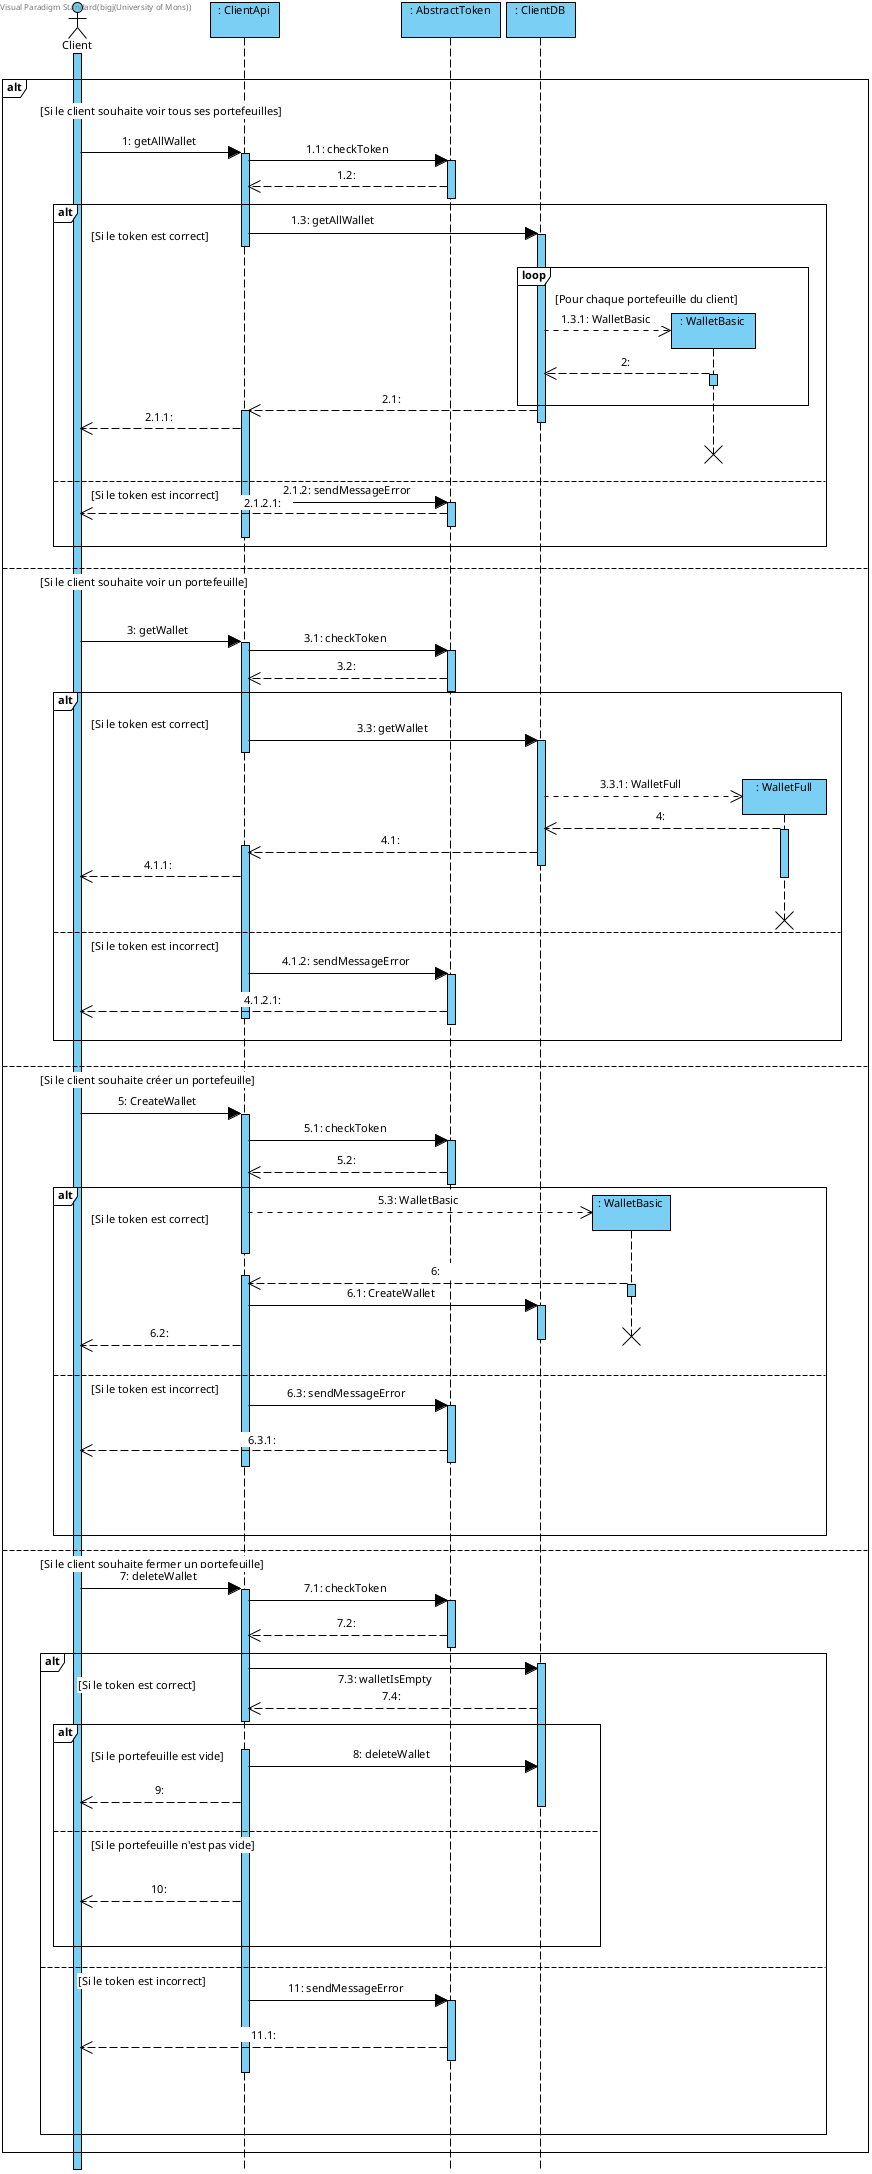
\includegraphics[height = 1.2\textwidth]{Base/sequence/img/client/Voir les portefeuilles.png}
\end{figure}
\newpage

\subsection{Provider}

\begin{flushleft}
Tout d'abord, nous avons fait en sorte qu'un use case peut être représenté via un choix alternatif. Aussi, pour éviter de répéter la même chose dans le rapport, nous posons que toutes les méthodes liées à l'API appelleront la méthode \textbf{checkToken} de \textbf{AbstractToken} ce qui impliquera deux choix alternatifs : "Si le token est correct" et "Si le token est incorrect". Dans le dernier cas, on renverra un message d'erreur au fournisseur.
\end{flushleft}
\subsubsection{Gestion des clients}
\begin{flushleft}
Commençons par le use case "voir ses clients". Afin qu'un fournisseur puisse voir ses clients, il lui suffit d'appeler la méthode \textbf{getAllHisClients} dans la classe \textbf{ProviderApi} et \textbf{ProviderDB}. Etant donné qu'on retourne une collection d'objet \textbf{ClientBasic}. Nous devons utiliser une boucle. Pour voir un seul de ses clients, il lui suffit d'appeler la méthode \textbf{getClient}.
\end{flushleft}

\begin{flushleft}
Passons maintenant au use case "supprimer un client". Pour faire cela, la méthode \textbf{deleteClient} sera utilisée. Par conséquent, une notification sera envoyée au client ce qui nous oblige à faire appel à la méthode \textbf{createNotification}. 
\end{flushleft}

\begin{flushleft}
Pour ajouter un client, cela se fera par le biais d'une proposition du fournisseur au client. Ceci faisant appel à la méthode \textbf{providerProposeContract}. Nous posons comme hypothèse que le client n'a aucun contrat en cours avec le fournisseur. 
\end{flushleft}

\begin{flushleft}
Pour qu'un fournisseur puisse ajouter des clients. Il doit d'abord avoir accès à tous les clients de l'application. Ceci se fera par la méthode \textbf{getAllClients}. De la même manière que voir "ses clients", nous utiliserons une boucle.  
\end{flushleft}

\newpage
\begin{figure}[h]
    \centering
    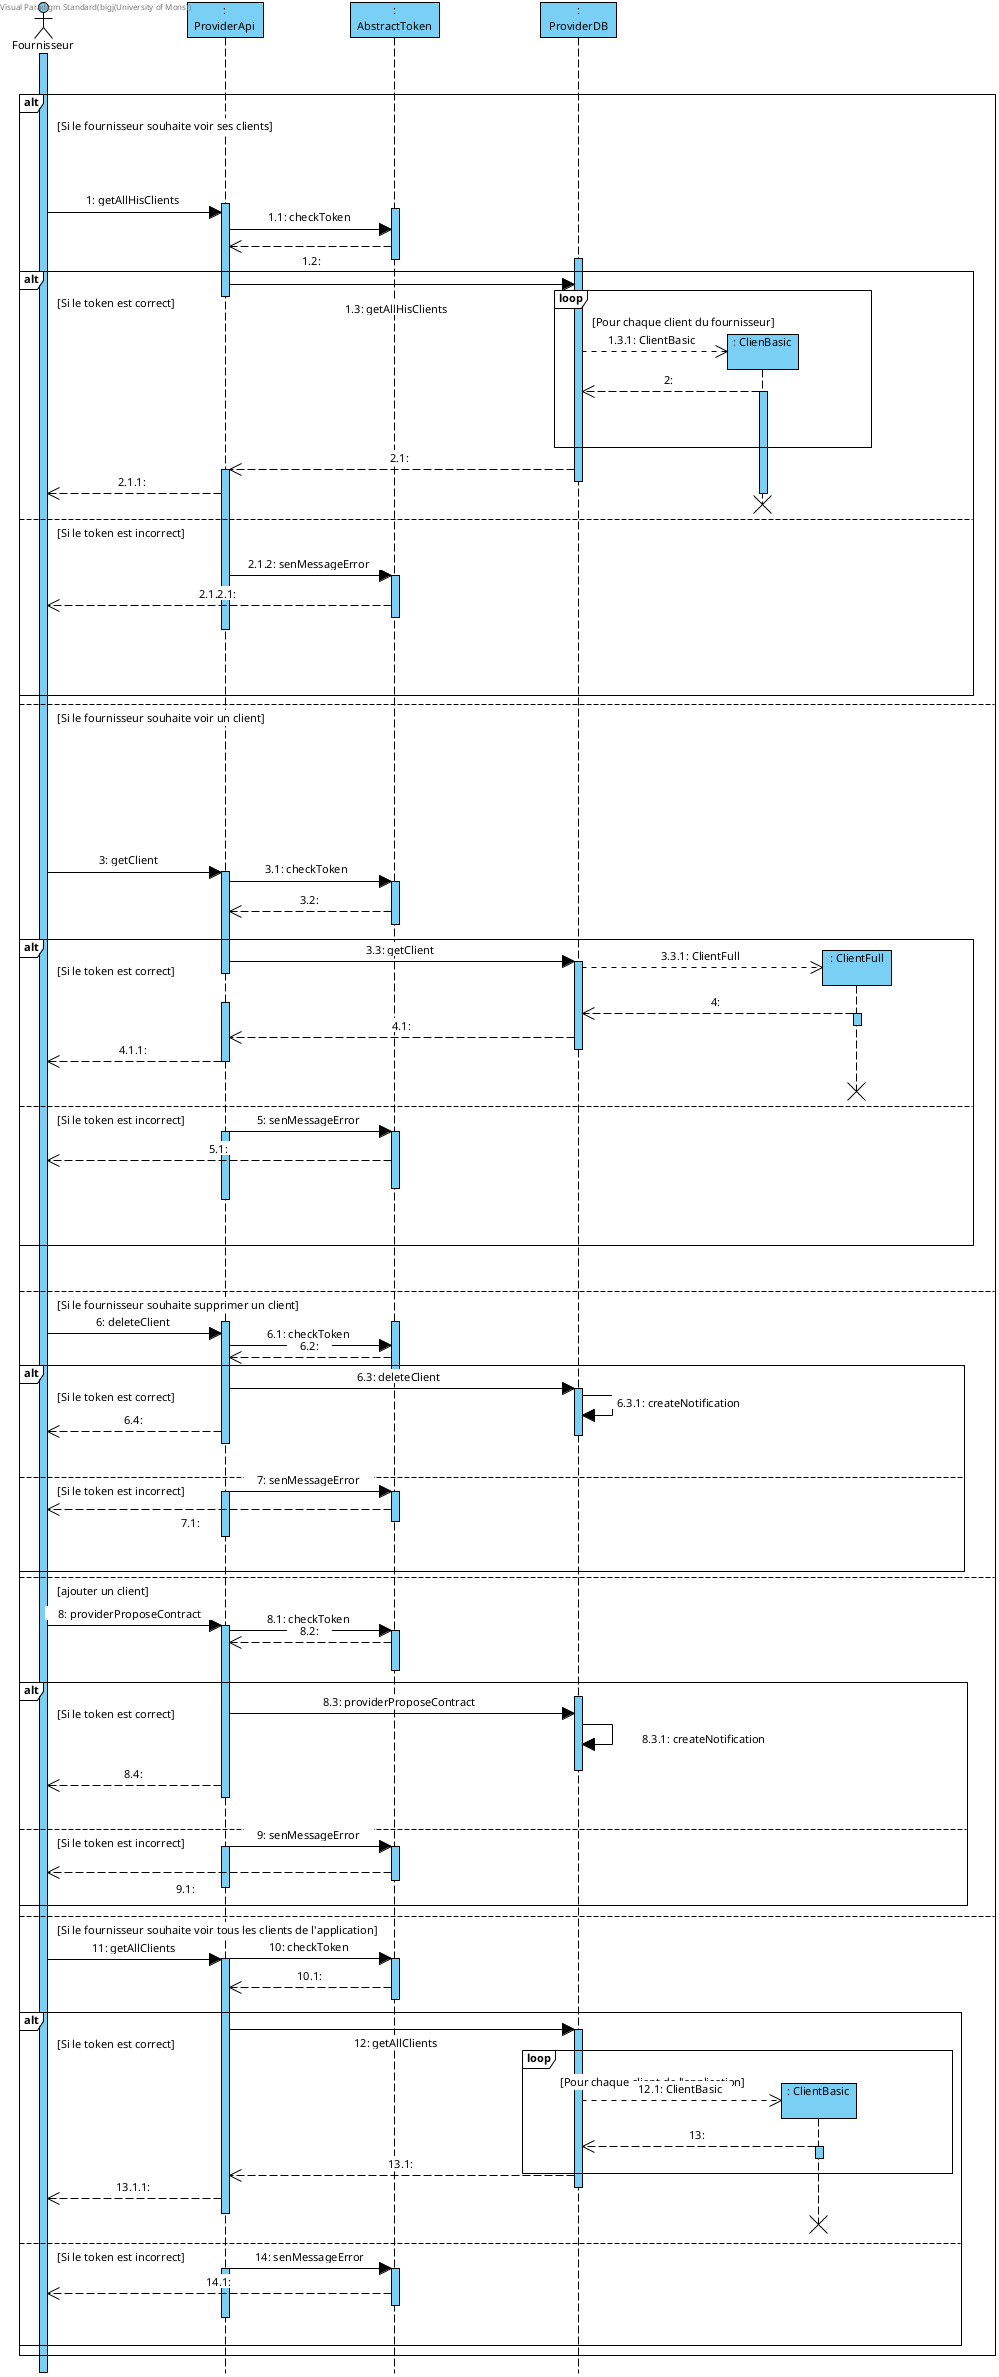
\includegraphics[height = 1\textwidth]{Base/sequence/img/fournisseur/voir_ses_clients.png}
\end{figure}
\newpage
\subsubsection{Gestion des propositions}
\begin{flushleft}
Avant de parler des diagrammes de séquence de cette partie. Nous avons choisi de mettre les contrats d'un fournisseur et ses propositions dans les use cases parlant des contrats. De plus, seules les propositions seront abordées dans cette partie étant donné qu'un contrat sera commun au fournisseur et au client(section \ref{CONTRATS},page \pageref{CONTRATS}).
\end{flushleft}

\begin{flushleft}
Pour commencer, nous allons regarder comment le fournisseur peut avoir accès à toutes ses propositions. Pour cela, il devra utiliser la méthode \textbf{getAllProposals}. De plus, une boucle permettra de récupérer tous les objets. Si le fournisseur veut avoir plus de précision sur une de ses propositions, alors il aura juste besoin d'apeller la méthode \textbf{getProposal} en ayant l'identifiant de la proposition au préalable.
\end{flushleft}
\begin{flushleft}
Après ça, Si le fournisseur veut ajouter une proposition. La méthode \textbf{addProposal} sera utilisée. Il faudra néanmoins créer un objet \textbf{ProposalFull} qui sera ensuite ajouté par la précédente méthode à la base de données. 
\end{flushleft}

\begin{flushleft}
Ensuite, si le fournisseur souhaite modifier les paramètres d'une de ses propositions. Il n'aura qu'à faire un nouvel objet qui servira de "remplacant" à l'ancienne proposition. La méthode \textbf{changeProposal} sera appelée par la suite pour faire le changement des paramètres directement dans la base de données. A noter que modifier les paramètres d'une proposition revient à changer les contrats avec les clients qui ont pris cette proposition. De ce fait, une notification sera envoyée via la méthode \textbf{createNotification}.
\end{flushleft}

\begin{flushleft}
Pour finir cette partie, nous allons parler de comment fonctionne la procédure pour supprimer une proposition. Nous avons juste à faire appel à la méthode \textbf{deleteProposal}. De manière similaire au fait de modifier, supprimer implique la supression des contrats des clients ayant comme base cette proposition ce qui implique l'envoi d'une notification par la méthode \textbf{createNotification}.
\end{flushleft}

\newpage
\begin{figure}[h]
    \centering
    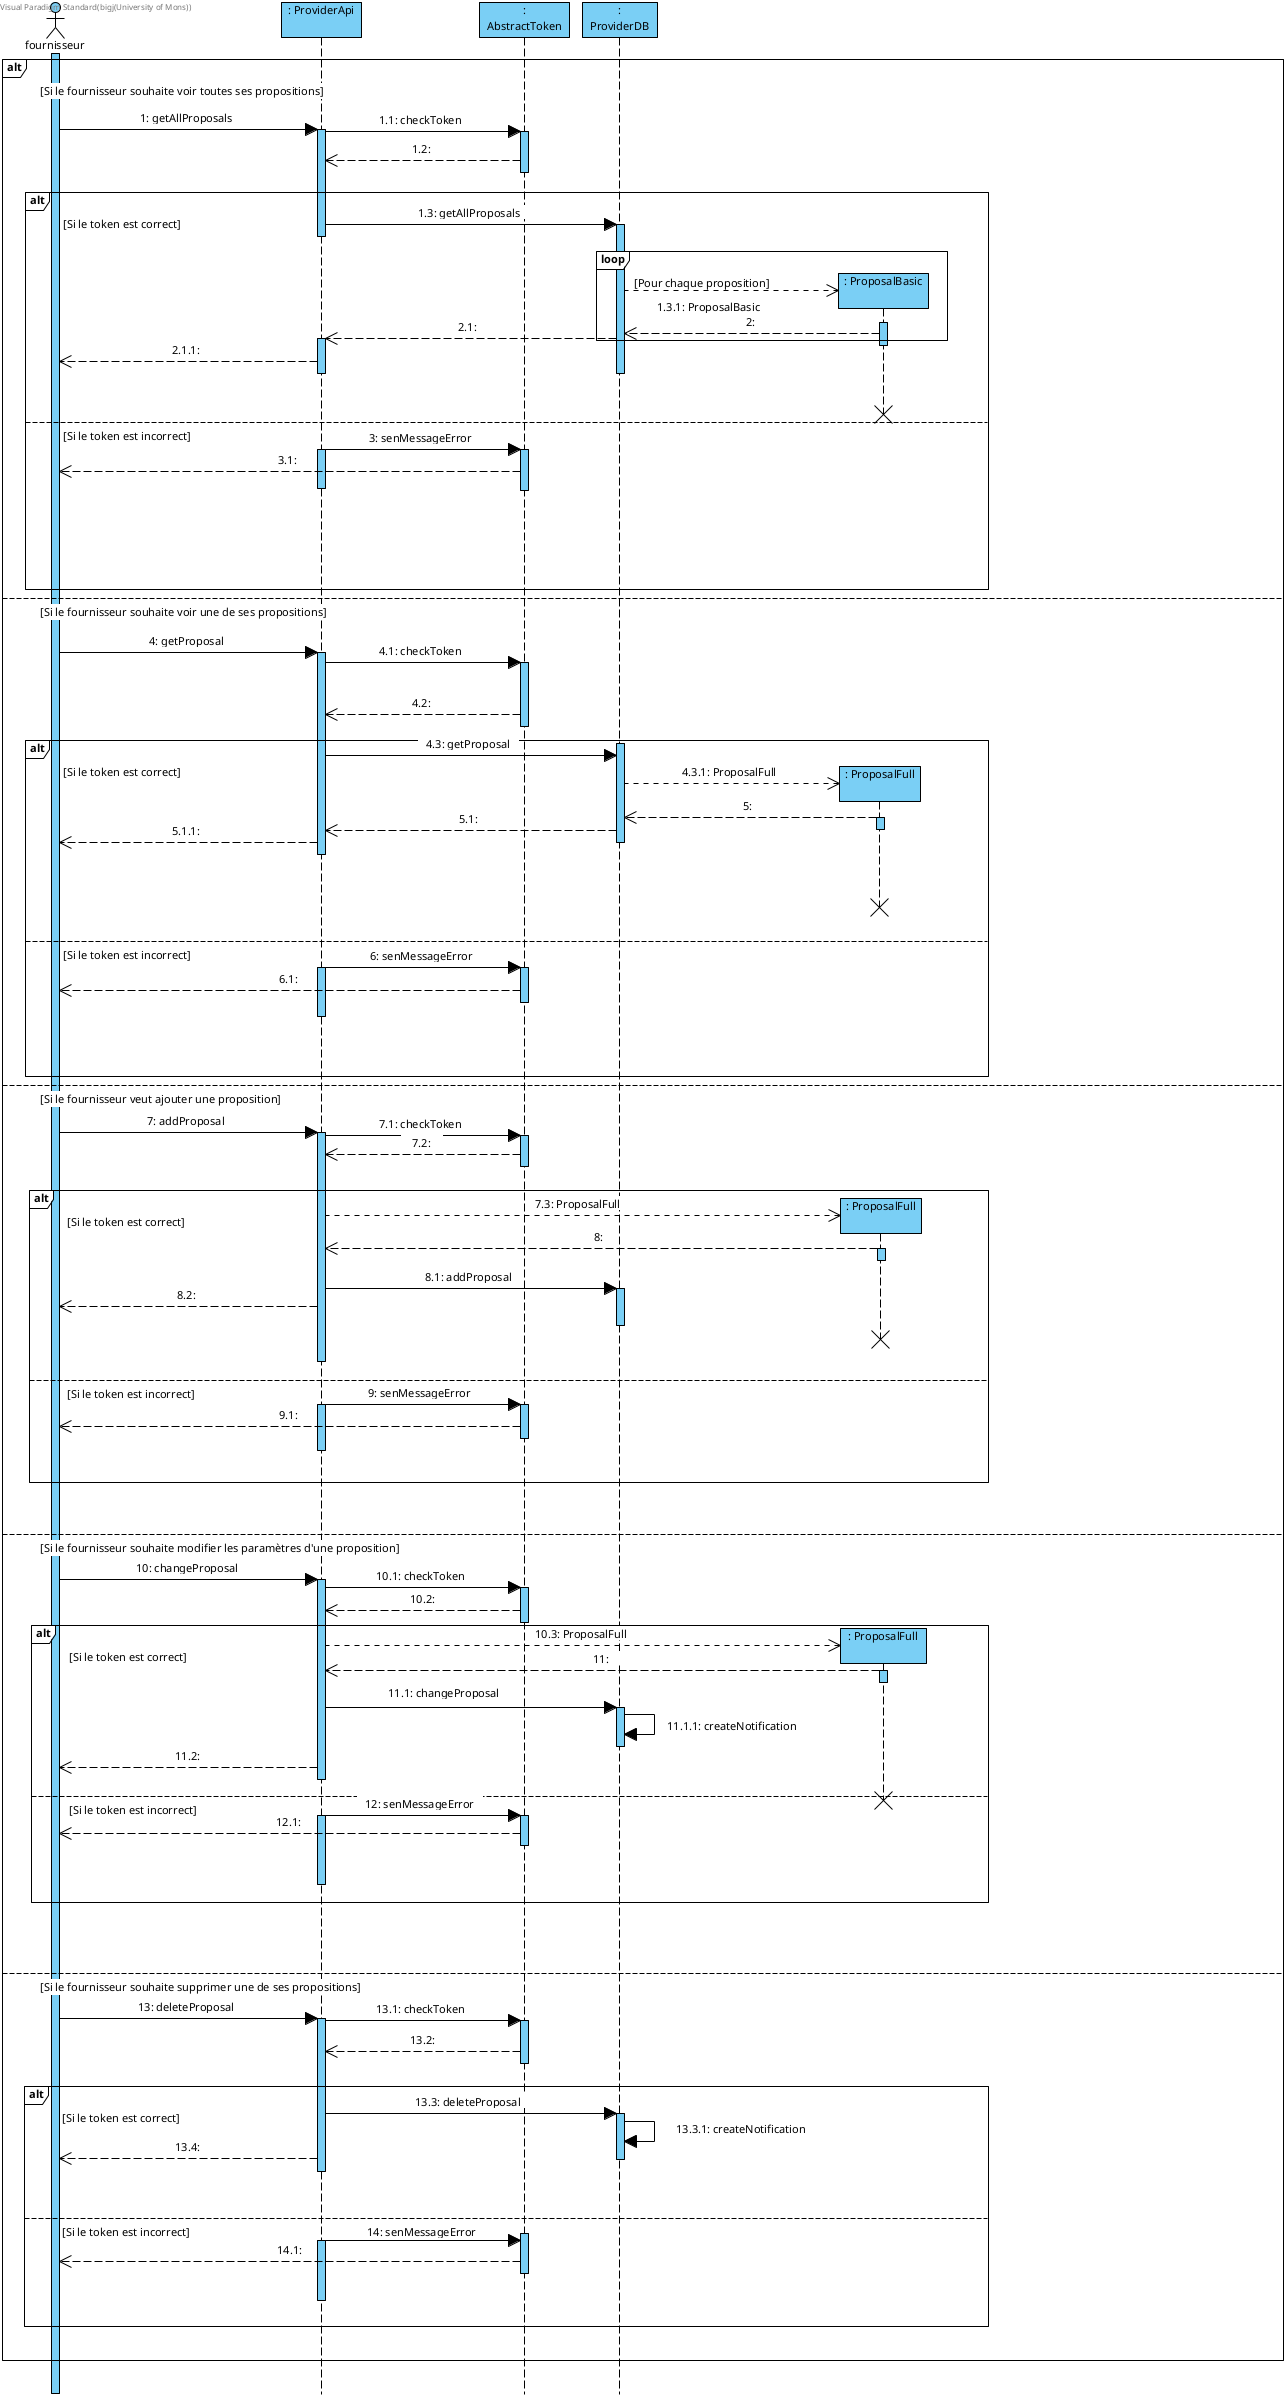
\includegraphics[height = 0.9\textwidth]{Base/sequence/img/fournisseur/voir les propositions.png}
\end{figure}

\newpage
\subsubsection{Gestion de la consommation}
\begin{flushleft}
Cette sous-sous-section parlera de la gestion de la consommation d'un client par le fournisseur. A noter que le fait pour un fournisseur de voir la consommation de ses clients est la même procédure qu'un client qui va voir ses consommations à l'exception qu'un fournisseur ne peut voir la consommation créée par le client liée à son contrat.     
\end{flushleft}

\begin{flushleft}
Tout d'abord, le fournisseur souhaitant supprimer une donnée de consommation devra passer par la méthode \textbf{deleteConsumption} de l'API. De plus, il aura besoin d'un objet \textbf{Calendar} ne contenant que l'année, le mois et le jour. Après ça, il pourra supprimer la donnée qu'il souhaite avec la méthode portant le même nom que celle de l'API. Une notification sera envoyée au client avec la méthode \textbf{createNotification}.
\end{flushleft}

\begin{flushleft}
Ensuite, si le fournisseur souhaite supprimer toutes les données de consommation d'un client. Il aura juste besoin de la méthode \textbf{deleteAllConsumption}. De même que le paragraphe du dessus, une notification sera créée.
\end{flushleft}

\begin{figure}[h]
    \centering
    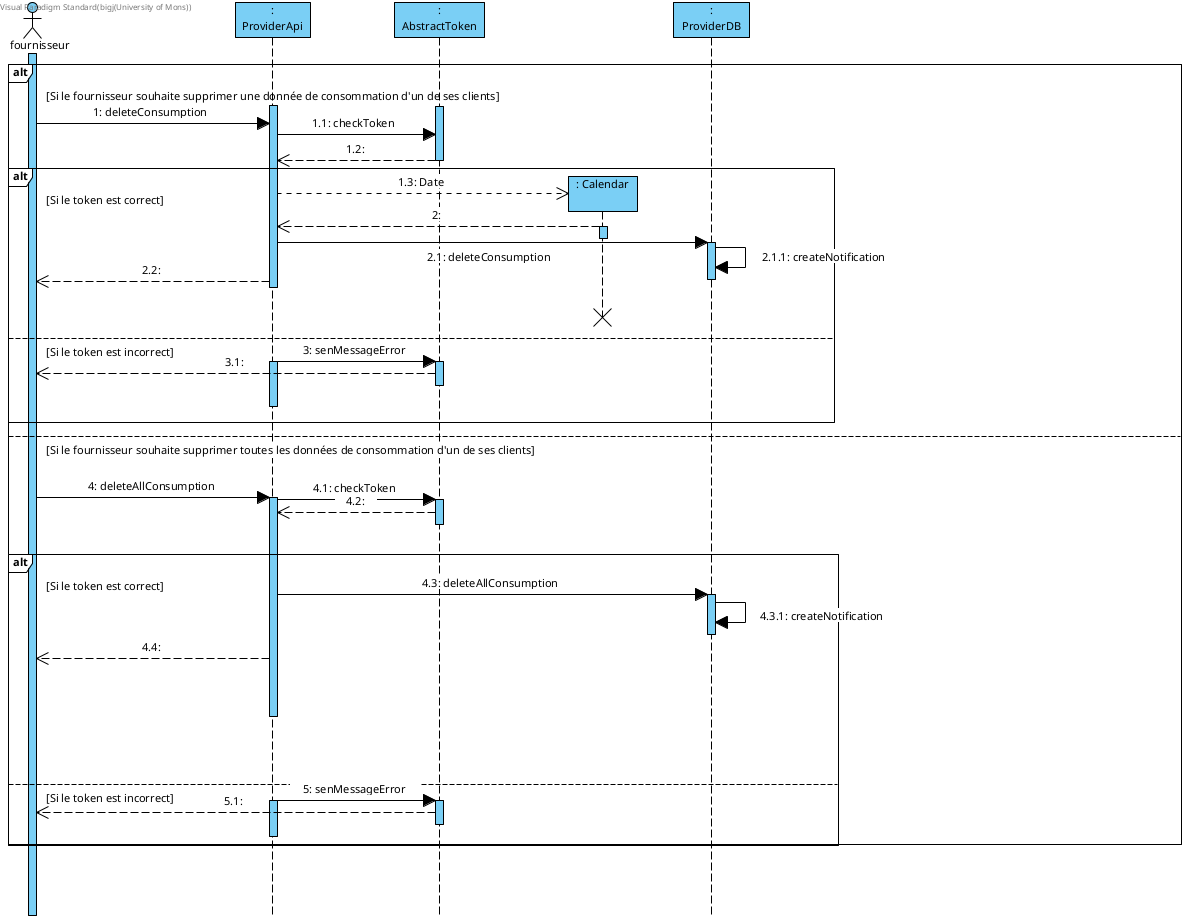
\includegraphics[height = 0.8\textwidth]{Base/sequence/img/fournisseur/gestion de la consommation.png}
\end{figure}

\section{Interface}

\subsection{Introduction}

Nous avons réalisé notre interface principalement sur base de nos usecases et overview diagrams ainsi que les choix effectués concernant la base de données et le class diagram.

\begin{flushleft}
Cette manière de procéder nous a permis de structurer nos idées afin de fournir l'interface la plus intuitive possible.
\end{flushleft}

\begin{flushleft}
De plus, nous avons décidé de séparer l'interface en \textbf{trois parties} :
\end{flushleft}

\begin{enumerate}[1.]
\item Le système de logs
\item L'interface client
\item L'interface fournisseur
\end{enumerate}

\begin{flushleft}
ce qui nous semblait plus approprié étant donné que nous devons obtenir deux applications distinctes, une pour le fournisseur et l'autre pour le client.
\end{flushleft}

\begin{flushleft}
Il est important de noter que nous avons utilisé le logiciel "Figma" pour réaliser ces maquettes.
\end{flushleft}

\newpage
\subsection{Système de logs}
Sur la page principale de connexion, l'utilisateur devra préciser s'il est client ou fournisseur en cochant la case apppropriée et pourra également changer de langue s'il le souhaite.
\begin{flushleft}
Il pourra dès lors entrer ses informations et \textbf{se connecter}.
\end{flushleft}

\begin{flushleft}
Cependant s'il a \textbf{oublié son mot de passe}, un bouton sera prévu à cet effet.
Ce dernier enverra l'utilisateur sur une nouvelle page où il devra inscrire le code qu'il aura reçu par mail et son nouveau mot de passe.
\end{flushleft}

\begin{flushleft}
Un bouton "Submit" aura pour but de confirmer ce que l'utilisateur a entré et un bouton "Back" sera présent si jamais ce dernier veut retourner en arrière.
\end{flushleft}


\begin{flushleft}
S'il n'a pas encore de compte, l'utilisateur aura la possibilité d'en \textbf{créer un nouveau}. 
Le sytème fonctionnera comme la connexion expliquée précédemment.
\end{flushleft}

\begin{flushleft}
La seule différence réside lorsque ce dernier appuiera sur le bouton "Create an account". 
L'utilisateur sera alors envoyé sur une nouvelle page où on lui demandera de confirmer la création de son compte en entrant le code qu'il aura reçu par mail pour plus de sécurité.
\end{flushleft}

\begin{flushleft}
Pour finir, de la même manière que pour le changement de mot de passe, un bouton "Finish" aura pour but de confirmer ce que l'utilisateur a entré et un bouton "Back" sera présent si jamais ce dernier veut retourner en arrière.
\end{flushleft}

\begin{flushleft}
En outre, l'utilisateur pourra demander qu'on lui renvoie un mail si le précédent n'est pas reçu.
\end{flushleft}\

\newpage
\begin{figure}
    \centering
    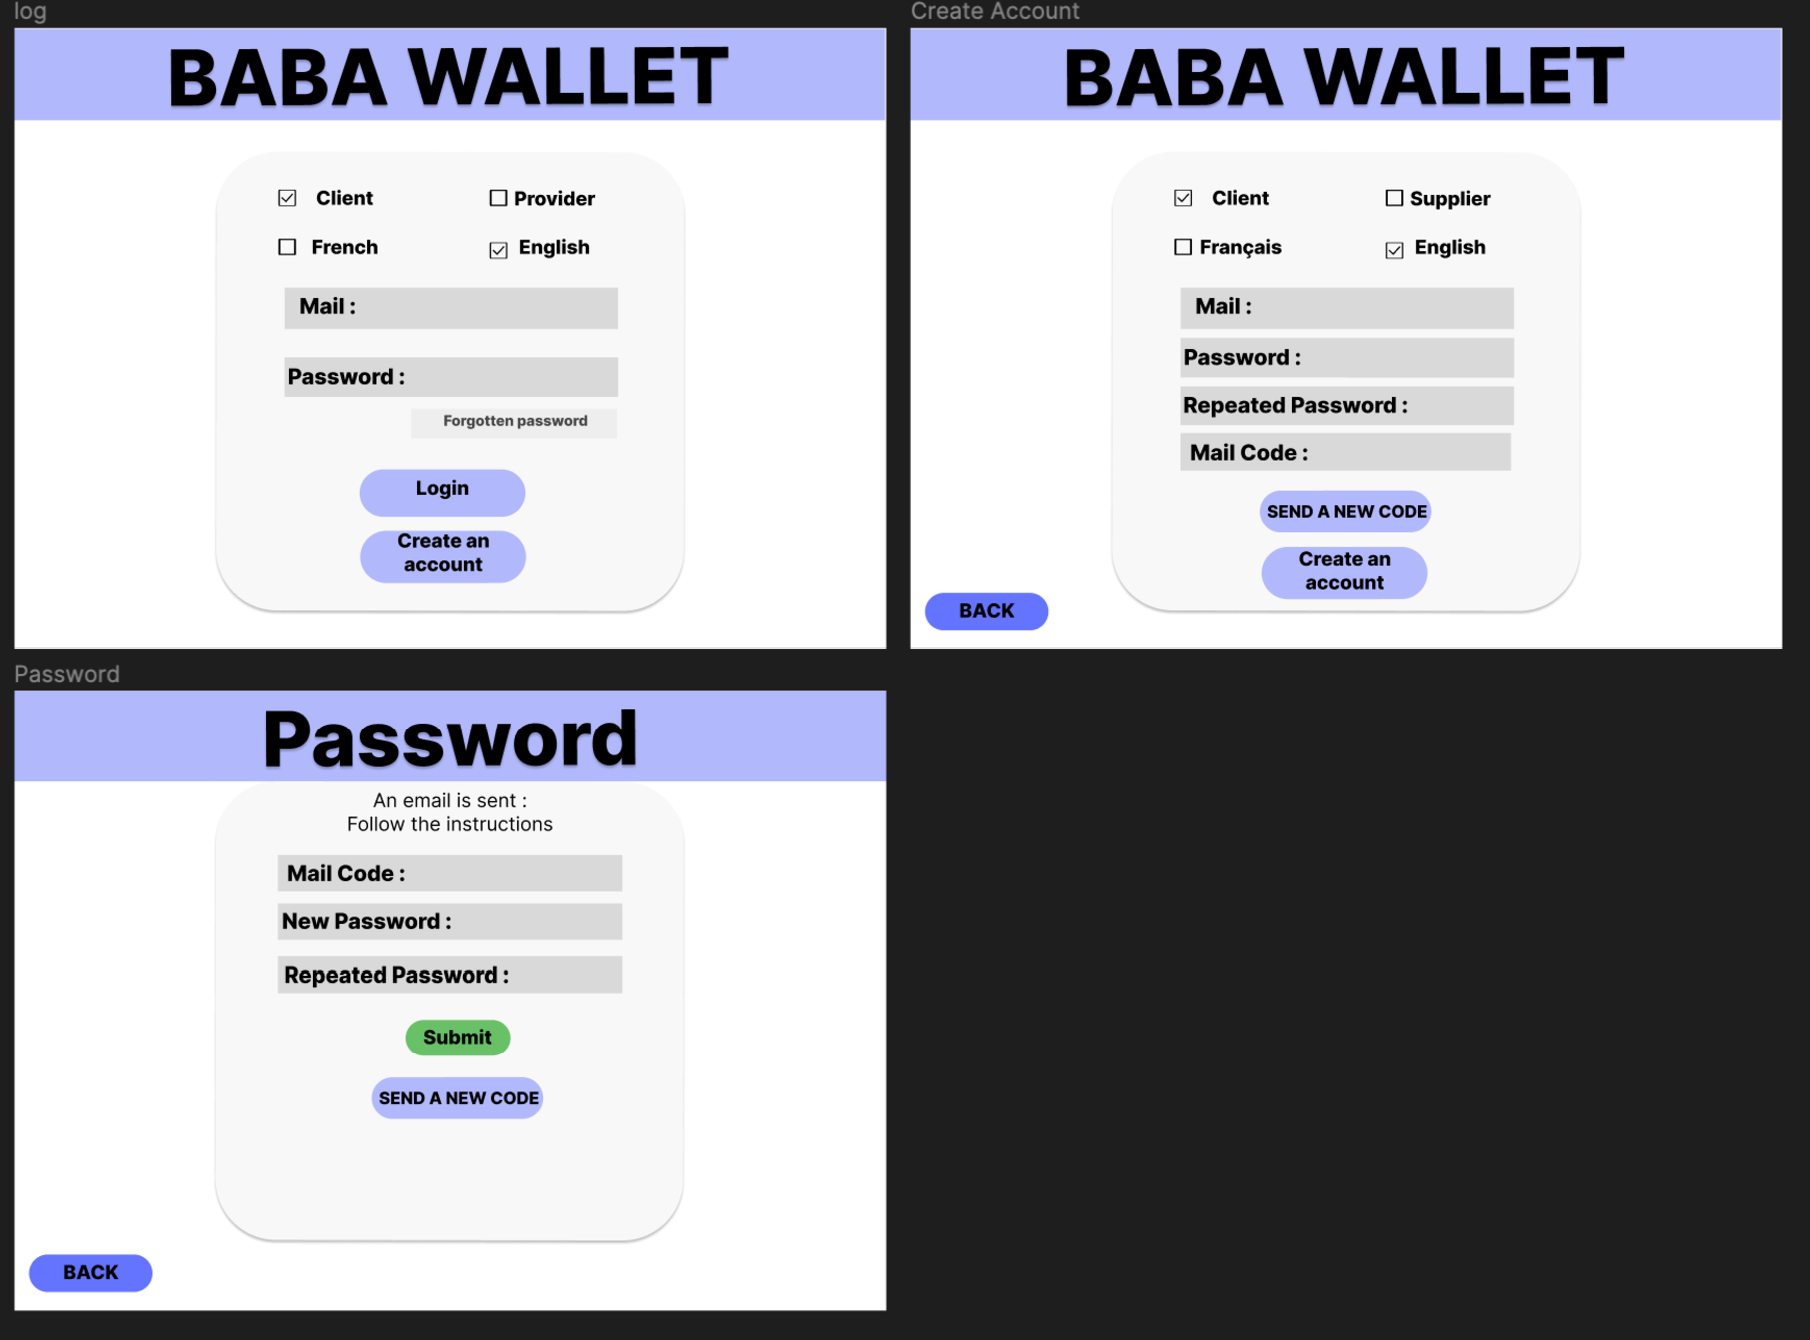
\includegraphics[width = 1\textwidth]{Base/interface/img/Log.pdf}
\end{figure}
\newpage
\subsection{Points communs}
Les points communs entre l'interface client et fournisseur sont
\begin{enumerate}
\item \textbf{Les notifications :}\newline
L'utilisateur verra le fournisseur ou client en question, le contexte et le contrat lié à la notification.\newline
Il pourra également observer plus en détail le contrat avec le bouton "See", marquer commme lue les notifications grâce au bouton "OK" et les accepter ou refuser dans le cadre d'une demande.\newline
En outre, la possibilité d'actualiser lui-même s'il le désire lui est laissée.
\item \textbf{Les paramètres :}\newline
Concernant le changement de mot de passe, cela se déroule exactement de la même manière que dans le système de logs.
Pour la langue, l'utilisateur pourra en ajouter, choisir sa préférée et changer celle étant active.\newline
Dans tous les cas, ce dernier sera conduit sur une page où il aura la possibilité de chercher une langue et ensuite soit de la télécharger, soit de la choisir en fonction du contexte.
\end{enumerate}



\newpage
\subsection{Interface client}

Lorsqu'un client se connectera, il arrivera sur la page d'acceuil ou plus précisément "Home".
\begin{flushleft}
Ce dernier aura alors les possibilités suivantes :
\end{flushleft}
\begin{enumerate}
\item Voir ses portefeuilles ("Wallets")
\item Voir ses contrats ("Your contracts")
\item Voir ses notifications
\item Voir les fournisseurs et contrats relatifs ("See new contracts")
\item Se déconnecter
\item Aller sur la page des paramètres
\end{enumerate}

\begin{flushleft}
Il est important de noter que ce n'est qu'à partir de ces six pages que le client pourra revenir sur la page "Home" étant donné le choix effectué dans notre overview diagram.
\end{flushleft}

\begin{flushleft}
Néanmoins, ce dernier aura la possibilité de revenir en arrière à l'aide du bouton "Back" lorsqu'il sera sur des "sous-pages" de ces six sections principales.
\end{flushleft}

\newpage
\begin{flushleft}
Nous pouvons maintenant commencer par l'option \textbf{"Voir ses portefeuilles" ("Wallets")} :
\end{flushleft}

\begin{flushleft}
Le client pourra à partir d'ici voir une liste reprenant tous les portefeuilles qu'il aura créé précédement. 
\end{flushleft}
\begin{flushleft}
Chaque rectangle représentant un portefeuille comprend :
\end{flushleft}
\begin{enumerate}
\item Le nom du portefeuille
\item Le nom du propriétaire du portefeuille
\item L'adresse associée au portefeuille
\end{enumerate}
\begin{flushleft}
Le bouton "Go" permettra de voir plus en détail un portefeuille et le bouton "+" sur le rectangle vide donnera la possibilité au client d'ajouter un nouveau portefeuille.
\end{flushleft}
\begin{flushleft}

Lorsqu'il souhaitera \textbf{voir plus en détail un portefeuille}, le client aura accès au nom du portefeuille, au nom du propriétaire du portefeuille et à l'adresse associée au porteuille comme sur la page précédente.
\end{flushleft}
\begin{flushleft}
Toutefois d'autres actions lui seront possibles :
\end{flushleft}
\begin{enumerate}
\item Voir ses dernières consommations
\item Voir les contrats associés
\item Voir les contrats associés en détail (Bouton "Go")
\item Ajouter des consommations (Bouton "Add consumptions")
\item Fermer définitivement le portefeuille (Bouton "Close the Wallet")
\end{enumerate}

\begin{flushleft}
Le bouton "Go" concernant les contrats associés l'amènera sur une page montrant le contrat que nous expliquerons prochainement.
\end{flushleft}

\begin{flushleft}
Le bouton \textbf{"Add consumptions"} l'entraînera vers une page où il pourra voir ses données de consommations en graphique ou en tableau à l'aide des deux boutons placés en haut de la page.
\end{flushleft}
\begin{flushleft}
Le réctangle gris les représentent et il pourra également séléctionner dans ce dernier s'il souhaite voir les données mensuellement, hebdomadairement,...
\end{flushleft}
\begin{flushleft}
Le client pourra également s'il le désire exporter ses données.
Nous pouvons noter que ce dernier exportera les données présentent dans le tableau gris au moment où il appuiera sur le bouton "Export".
\end{flushleft}
\begin{flushleft}
En ce qui concerne le changement et l'ajout de consommation, celui-ci devra entrer la date correspondante, le type d'énergie et la valeur associée et devra ensuite confirmer ses modifications grâce aux boutons "Change" et "Add".
\end{flushleft}

\begin{flushleft}
\textbf{Le bouton "+"} mentionné précédemment servant à ajouter un nouveau portefeuilles est connecté à une page qui lui demandera d'écrire le nom et l'adresse du nouveau portefeuille.
\end{flushleft}

\begin{flushleft}
Cette manière de procéder est liée au fait que nous avons décidé qu'un portefeuille doit être créé avant d'associer un contrat à ce dernier.
\end{flushleft}

\begin{flushleft}
La deuxième option est la suivante : \textbf{"Voir ses contrats" ("Your contracts")}
\end{flushleft}

\begin{flushleft}
Une fois sur cette page, le client aura accès à sa liste de contrats et il pourra rechercher un contrat spécifique en tapant le code "EAN" ou le nom du fournisseur.
\end{flushleft}

\begin{flushleft}
Les informations basiques qu'il verra sur chaque ligne de la liste sont le fournisseur et le type d'énergie.
\end{flushleft}

\begin{flushleft}
Lorsqu'il cliquera sur le \textbf{bouton "Go"} la nouvelle page lui offrira les informations suivantes : le type d'énergie et le fournisseur de la même manière que sur la page précédente.
\end{flushleft}
\begin{flushleft}
Les nouvelles informations disponibles sont les suivantes :
\end{flushleft}
\begin{enumerate}
\item Le nom du contrat
\item Le portefeuille associé (Le code "EAN" ainsi que l'adresse)
\item La localisation (du contrat)
\item Le prix basique
\item Le prix dépendant du jour et la nuit
\item Le taux fixe ou variable
\item Les heures creuses
\item La date d'ouverture du contrat
\item La date de fermeture du contrat
\end{enumerate}
\begin{flushleft}
Il pourra aussi fermer le contrat par le bouton "Close the contract".
\end{flushleft}

\newpage

\begin{flushleft}
La troisième et dernière section est \textbf{"Voir les fournisseurs et contrats relatifs ("See new contracts")"}
\end{flushleft}
\begin{flushleft}
Sur cette page, le client pourra voir une liste reprenant les noms des fournisseurs, les types d'énergies et la localisation pour chaque contrat.
\end{flushleft}
\begin{flushleft}
Pour lui rendre la tâche de recherche plus facile, nous avons mis à sa disposition une sélection sur le côté droit.
Cette dernière permettra de choisir le type d'énergie souhaité (Electricité, gaz et eau) ainsi que la localisation.
\end{flushleft}

\begin{flushleft}
Le \textbf{bouton "Go"} l'amènera sur les informations liées à un nouveau contrat :
\end{flushleft}
\begin{enumerate}
\item Le fournisseur
\item Le type d'énergie
\item La localisation (du contrat)
\item Le prix basique
\item Le prix dépendant du jour et la nuit
\item Le taux fixe ou variable
\item Les heures creuses
\item Le type de compteur
\end{enumerate}
\begin{flushleft}
Pour confirmer sa demande de contrat, le client devra entrer le nom du portefeuille auquel il souhaite l'associer ainsi que le code "EAN" et appuyer sur le bouton "Submit".
\end{flushleft}

\begin{flushleft}
Nous ne reviendrons pas sur les points "Voir les notifications" et "Les paramètres", ces derniers étant expliqués dans les points communs. 
\end{flushleft}

\begin{figure}
    \centering
    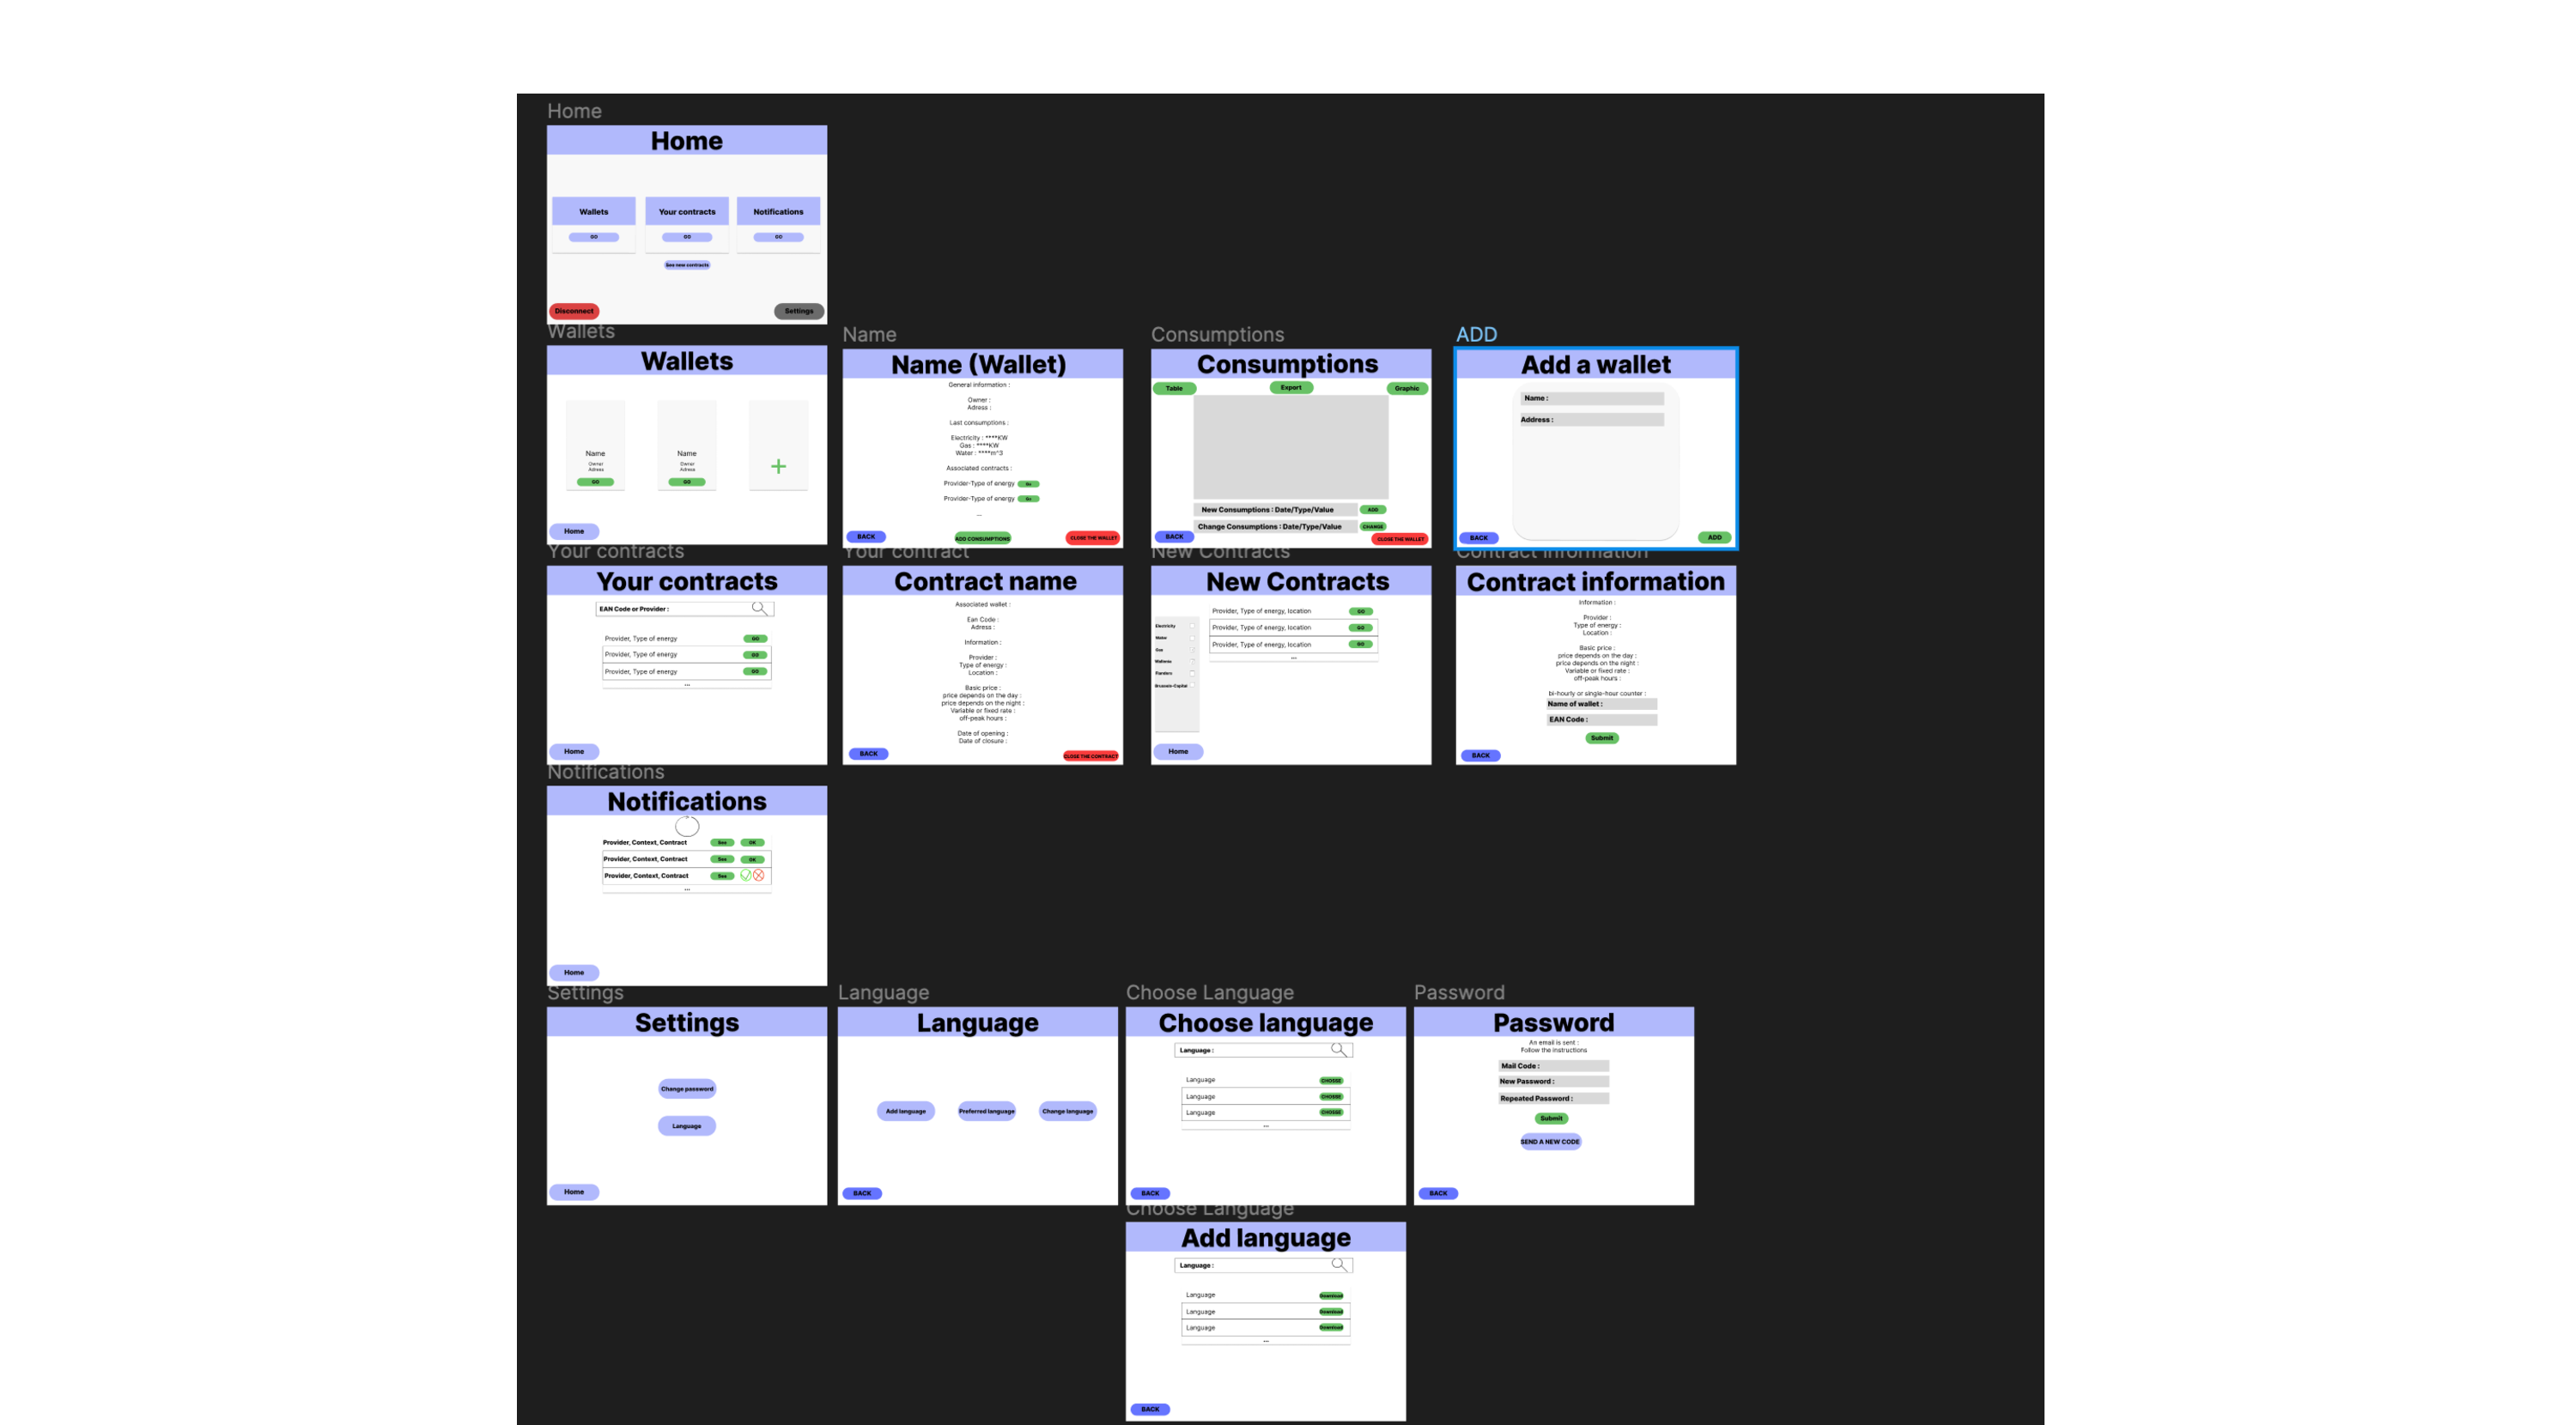
\includegraphics[width = 1\textwidth]{Base/interface/img/Client.pdf}
\end{figure}

\newpage
\subsection{Interface fournisseur}

Lorsqu'un fournisseur se connectera, il arrivera sur la page d'acceuil ou plus précisément "Home".
\begin{flushleft}
Ce dernier aura alors les possibilités suivantes :
\end{flushleft}
\begin{enumerate}
\item Voir ses clients ("Your clients")
\item Voir ses contrats ("Your contracts")
\item Voir ses notifications
\item Se déconnecter
\item Aller sur la page des paramètres
\end{enumerate}

\begin{flushleft}
Tout comme pour l'interface client, il est important de noter que ce n'est qu'à partir de ces six pages que le fournisseur pourra revenir sur la page "Home" étant donné le choix effectué dans notre overview diagram.
\end{flushleft}

\begin{flushleft}
Néanmoins, ce dernier aura la possibilité de revenir en arrière à l'aide du bouton "Back" lorsqu'il sera sur des "sous-pages" de ces six sections principales.
\end{flushleft}

\newpage

\begin{flushleft}
La première section est \textbf{Voir ses clients ("Your clients")}
\end{flushleft}

\begin{flushleft}
Le founisseur pourra à partir d'ici voir une liste reprenant tous les noms de ses clients ainsi que leurs adresses mails. 
\end{flushleft}

\begin{flushleft}
\textbf{Le bouton "Go"} lui permettra de voir plus en détail un client, il aura accès à :
\end{flushleft}
\begin{enumerate}
\item Son nom
\item Son adresse mail
\item Les contrats lui étant associés (Nom du contrat, code "EAN", le type d'énergie, la dernière consommation) : \newline
Le bouton "Go" lui donnera la possibilité de voir plus en détail le contrat de la même manière que lorsqu'un client souhaite voir ses contrats.\newline
Il aura la faculté de supprimer un contrat et voir les consommations.\newline
Contrairement au client, il ne pourra pas ajouter de nouvelles données de consommations mais simplement les modifier et les supprimer et ne pourra pas exporter les données mais en importer.
\item La suppresion d'un client (Bouton "Delete Client")
\end{enumerate}

\begin{flushleft}
Le \textbf{bouton "Add clients"} le mènera sur une page où il pourra sélectionner un contrat à envoyer à un possible nouveau client.
\end{flushleft}

\newpage

\begin{flushleft}
Passons à la deuxième section : \textbf{Voir ses contrats ("Your contracts")}
\end{flushleft}

\begin{flushleft}
Le founisseur pourra à partir d'ici voir une liste reprenant tous les noms de ses contrats, leurs types d'énergie ainsi que leurs localisations. 
\end{flushleft}

\begin{flushleft}
\textbf{Le bouton "Go"} lui donnera la possibilité de voir plus en détails ses contrats avec :
\end{flushleft}
\begin{enumerate}
\item Le nom du contrat
\item Le type d'énergie
\item La localisation (du contrat)
\item Le prix basique
\item Le prix dépendant du jour et la nuit
\item Le taux fixe ou variable
\item Les heures creuses
\item Le type de compteur
\end{enumerate}

\begin{flushleft}
Ce dernier aura également accès à la suppression du contrat et au changement du contrat fonctionnant comme \textbf{l'ajout de contrats (Bouton "Add contracts")} que nous allons expliquer ci-dessous.
\end{flushleft}

\begin{flushleft}
Lorsqu'un fournisseur souhaitera ajouter un contrat il devra entrer :
\end{flushleft}
\begin{enumerate}
\item Le nom du contrat
\item Le type d'énergie
\item La localisation (du contrat)
\item Le prix basique
\item Le prix dépendant du jour et la nuit
\item Les heures creuses
\item Le taux fixe ou variable
\item Le type de compteur
\end{enumerate}

\begin{flushleft}
Le bouton "Add" lui servira à valider la création du nouveau contrat.
\end{flushleft}

\begin{figure}
    \centering
    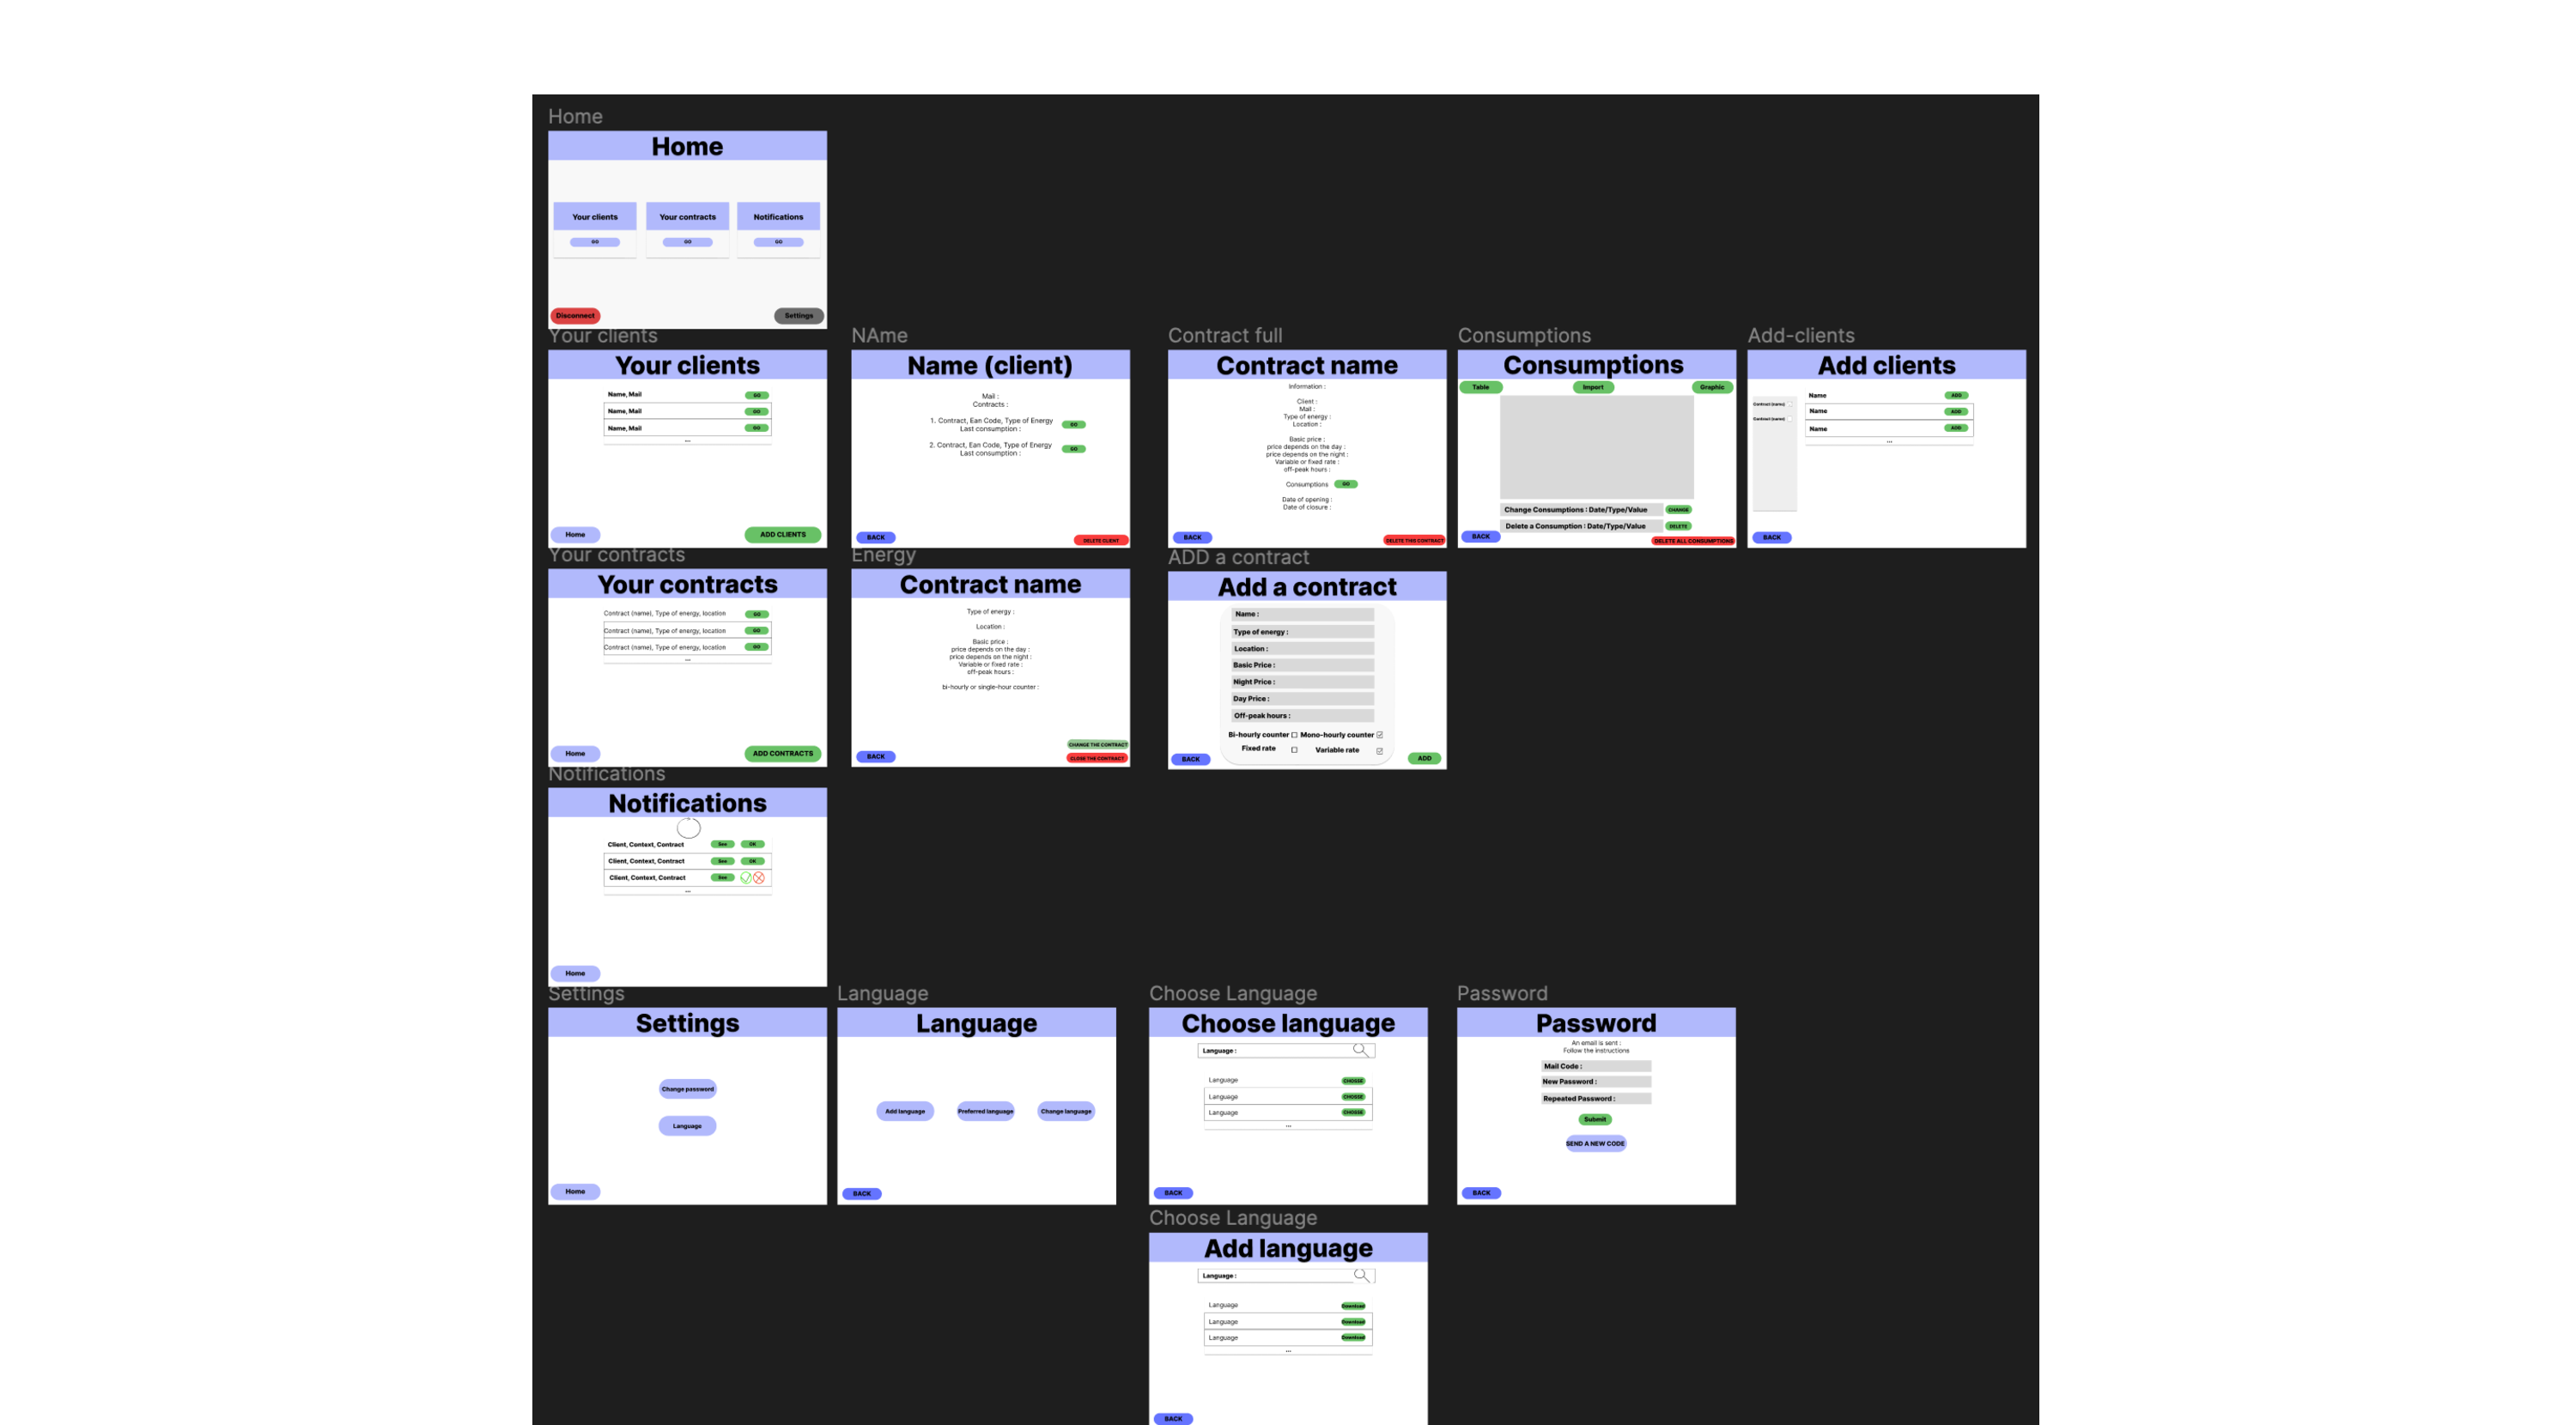
\includegraphics[width = 1\textwidth]{Base/interface/img/Supplier.pdf}
\end{figure}

\subsection{api-rest}

\begin{flushleft}
Pour terminer cette extension, il a fallu ajouter une requête API comme illustrée dans le diagramme de séquence sur \textbf{Comparer les données de consommations}. Nous retrouvons donc une requête API nommée \textbf{List Consumption Simulation} qui appellera la méthode \textbf{getConsumptionOfSimulation}. Pour cela, nous envoyons le token ainsi que la date de départ et la date de fin. Nous recevons en retour une liste de dates et de données de consommations journalières.
\end{flushleft}

\begin{flushleft}
Notez qu'il a fallu ajouter les paramètres concernant l'extension lors de la création d'un portefeuille et que nous pouvons également envoyer en plus lors d'une requête \textbf{List Wallets} pour que le client puisse voir toutes les informations liées à celui-ci.
\end{flushleft}

\begin{figure}[h]
\centering
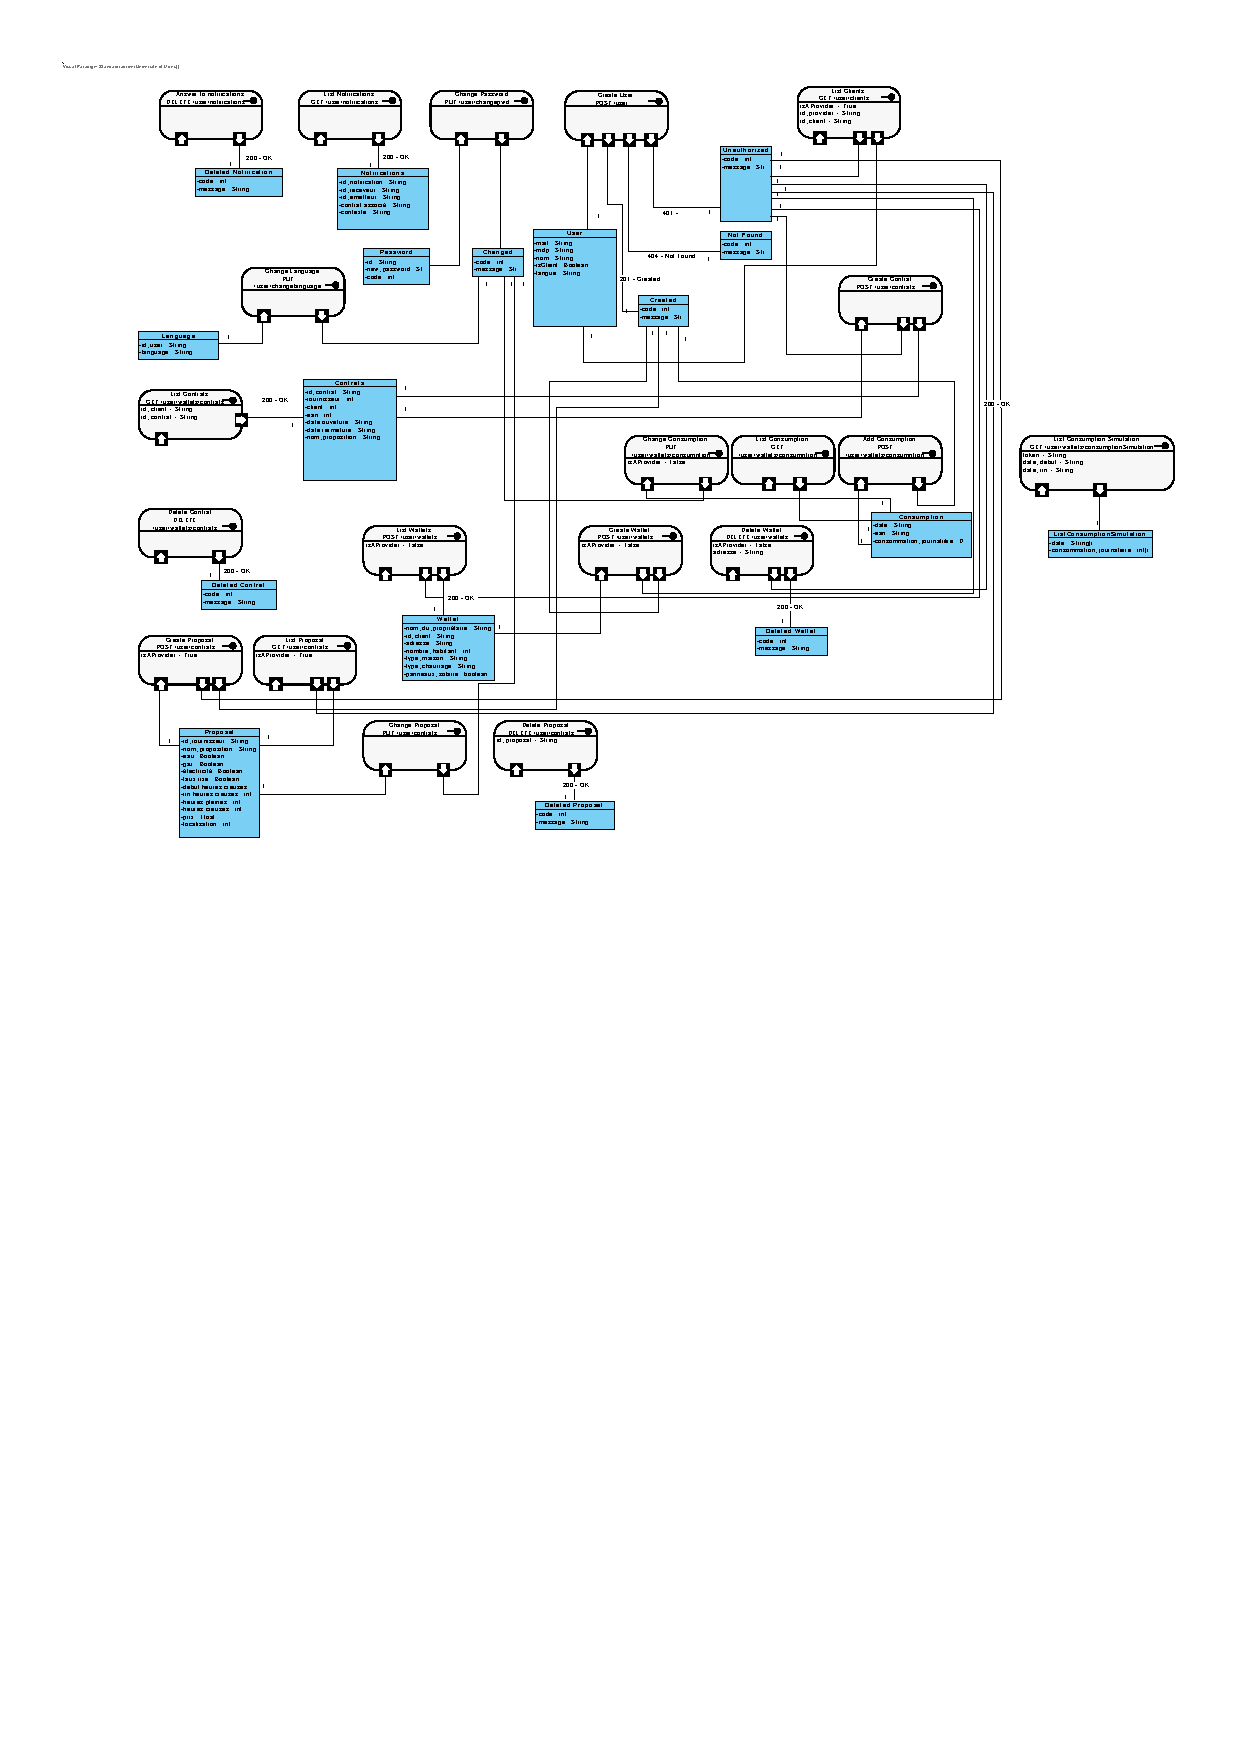
\includegraphics[width=1.3\textwidth]{extension-adrien/Api-rest/img/apirest.pdf}
\end{figure}

\section{Introduction-extension}

\begin{flushleft}
Pour plus de clarté, nous avons décidé de proposer un schéma de la base de données et de l'API pour les fonctionnalités de base.
\end{flushleft}

\begin{flushleft}
Ensuite, nous expliquerons comment ces schémas seront étendus respectivement pour chaque extension. 
\end{flushleft}

\begin{flushleft}
Notez donc que lors de l'implémentation, nous rassemblerons tout en une seule base de données et une seule API. 
\end{flushleft}

\end{document}
